%% Template for a preprint Letter or Article for submission
%% to the journal Nature.
%% Written by Peter Czoschke, 26 February 2004
%%

\documentclass[12pt]{article}

%% make sure you have the nature.cls and naturemag.bst files where
%% LaTeX can find them

\usepackage{scicite,graphicx,rotating}
\usepackage{times}


\title{Supplementary Material: 
``Climate change decouples drought from early winegrape harvests in Western Europe''}

%% Notice placement of commas and superscripts and use of &
%% in the author list
%/Users/bcook/Desktop/WINELIZZIE/MANUSCRIPT/figures_eps_png/SUPP_fig_12_JJA_clim_regplots.png

\author{Benjamin I Cook$^{1,2}$ \& Elizabeth M Wolkovich$^{3,4}$}


\begin{document}

\maketitle

\section*{Individual Site Analyses.}
\noindent Temperature is the dominant control on GHD in all seven regional series that make up the GHD-Core index (Supplementary Figures 4--10), and all temperatures regressions are highly significant ($p\le0.01$). For the period 1901--1980, the temperature sensitivities (regression slopes) across sites range from a minimum --2.59 days \textsuperscript{o}C\textsuperscript{--1} (SRv) to --8.41 days \textsuperscript{o}C\textsuperscript{--1} (Cha1). Significant moisture sensitivities (precipitation and PDSI regressions) are also found at most sites for this earlier time period: Als, Bor, Bur, Cha1, LLV. At SRv, precipitation and PDSI regressions against GHD during 1901--1980 are insignificant, while at Swi they are marginally ($p\le0.10$) significant.\\
\indent At all sites, GHD temperature sensitivities remain significant during the 1981--2007 interval, with no consistent pattern across sites towards either a strengthening or weakening of the relationship. By contrast, most sites show a substantial weakening of the two moisture sensitivities. Precipitation and PDSI regressions with GHD all become insignificant during 1981--2007 for Als, Bur, Cha1, and Swi. At LLV, the PDSI regression becomes insignificant and the precipitation regression weakens (although it is still significant with a $p=0.02$). At SRv, the relationship with moisture does not change; SRv is insensitive to moisture variability during 1901--1980 and remains so during 1981--2007. Only Bor slightly increases its' moisture sensitivity during the most recent period. Overall, the individual site level analyses support the conclusions drawn from analyses of the GHD-Core composite index, demonstrating an overall and large scale weakening of moisture controls on GHD in Western Europe.

\section*{Temperature versus Moisture Comparisons.}
\noindent A strong connection between soil moisture and warm season temperatures over the Mediterranean and Western Europe has been well established (ref XXXX), occurring primarily through the control of soil moisture on surface energy partitioning. In regions where evapotranspiration is limited by the supply of moisture at the surface, wetter soils will lead to increases in evapotranspiration and latent heat flux at the expense of sensible heating, keeping surface soil and air temperatures relatively cool. Conversely, if soils are dry, sensible heat fluxes will dominate, and soil and air temperatures will be higher. If these are the primary physics operating in our GHD-Core region, we would therefore expect negative relationships between temperature and precipitation or PDSI.\\
\indent Indeed, for both MJJ (Supplementary Figure 11) and JJA (Supplementary Figure 13) we can see significant negative relationships between both temperature and precipitation and PDSI during the 1901--1980 interval. The relationships are generally stronger during JJA, when solar energy inputs are larger and land-atmosphere interactions are expected to be stronger. During the more recent interval (1981--2007), the temperature moisture relationships generally weaken, especially during JJA. This suggests the temperature-moisture coupling strength in turn may be weakening with increased greenhouse gas warming.

%% TABLE: MEAN DATES
\begin{sidewaystable}
%\begin{table}
\small
\caption{\small Regional GHD series from DAUX used in construction of the GHD-Core composite series. Included are the codes for each site, their geographic locations (units of decimal degrees), and their mean harvest dates for various intervals.}
\centering
\begin{tabular}{| l l | r r | c c c c c p{5cm} |}
\hline
 \bf GHD Series & \bf Site Code & \bf Lat & \bf Lon & \bf 1600-1900 & \bf 1600-1980 & \bf 1901-1950 & \bf 1951-1980 & \bf 1981-2007 \\
\hline
Alsace	& Als & 48.17 & 7.28 & 282.81 & 281.87 & 272.12 & 287.16	 & 277.70 \\
Bordeaux	& Bor	& 45.18 & -0.75	& 269.01 & 	268.22	&  263.85 &  270.41 &  259.75\\
Burgundy	& Bur	& 47.32	& 5.04	& 269.92	& 270.07	& 269.44	& 272.58	& 262.15\\
Champagne 1	& Cha1	& 47.98	& 4.28	& 266.88	& 267.52	& 267.01	& 270.02	& 264.92\\
Low Loire Valley	& LLV	& 47.15	& 0.22	& 286.12	& 284.61	& 282.69	& 282.56	& 275.33\\
Southern Rhone Valley	& SRv	& 43.98	& 5.05	& 269.20	& 269.10	& 268.84	& 268.46	& 257.87\\
Switzerland (Lake Geneva)	& Swi	& 46.57	& 6.52	& 286.39	& 283.87	& 273.86	& 275.22	& 263.00\\
\hline
\end{tabular}
\end{sidewaystable}

%% TABLE: SERIAL COMPLETION
%\begin{sidewaystable}
\begin{table}
\small
\caption{\small For various intervals , the fraction of years for each regional GHD series for which observations are available.}
\centering
\begin{tabular}{l c c c c c}
\hline
 & \bf 1354-2007 & \bf 1600-1900 & \bf 1600-2007 & \bf 1800-2007 & \bf 1900-2007\\
\hline
Als	& 0.400612 & 0.578073 & 0.642157 & 0.836538	 & 0.824074\\
Bor	 & 0.500000 & 0.647841 & 0.737745 & 0.995192 & 0.990741\\
Bur & 	0.925076	& 0.996678	& 0.990196	& 0.985577	& 0.972222\\
Cha2	& 0.279817	& 0.259136	& 0.448529	& 0.879808	& 0.981481\\
LLV	& 0.310398	& 0.332226	& 0.497549	& 0.975962	& 0.962963\\
SRv	& 0.689602	& 0.970100	& 0.950980	& 0.942308	& 0.898148\\
Swi 	& 0.749235	& 1.000000	& 1.000000	& 1.000000	& 1.000000\\
\hline
\end{tabular}
\end{table}
%\end{sidewaystable}

%% TABLE: CROSS SITE CORRELATIONS
%\begin{sidewaystable}
\begin{table}
\small
\caption{\small Spearman's rank correlations (1600-2007) between each regional GHD series used in construction of the GHD-Core index.}
\centering
\begin{tabular}{c c c c c c c c}
\hline
& Als & Bor & Bur & Cha1 & LLV & SRv & Swi \\
\hline
Als	& 1	& 0.601045	& 0.573844	& 0.632206	& 0.502502	& 0.413751	& 0.604378\\
Bor & 0.601045 	& 1	& 0.622279		& 0.675208	& 0.712442 	& 0.321238 	& 0.547885\\
Bur &	0.573844	& 0.622279	& 1	& 0.798581	& 0.775801	& 0.542594	& 0.582605\\
Cha1	& 0.632206	& 0.675208	& 0.798581	& 1	 & 0.709044	& 0.346222	& 0.569444\\
LLV	& 0.502502	& 0.712442	& 0.775801	& 0.709044	& 1 & 0.456008 & 0.696642\\
SRv	& 0.413751	& 0.321238	& 0.542594	& 0.346222	& 0.456008	& 1	 & 0.525608\\
Swi	 & 0.604378	& 0.547885	& 0.582605	& 0.569444	& 0.696642	& 0.525608	& 1\\
\hline
\end{tabular}
%\end{sidewaystable}
\end{table}

%% TABLE: GHD ANOMALIES
%\begin{sidewaystable}
\begin{table}
\small
\caption{\small Anomalies in GHD, calculated relative to the baseline mean baseline calculated for 1600-1900. Also included are results for the GHD-Core index and GHD-All, composited from all 27 regional GHD series in DAUX. GHD-Core and GHD-All represent the composite average AFTER the anomalysing of the individual regional GHD series.}
\centering
\begin{tabular}{l c c c c c}
\hline
& \bf 1600-1900 & \bf 1600-1980 & \bf 1901-1950 & \bf 1951-1980 & \bf 1981-2007\\
\hline
Als	& 0	& -0.94 & -10.69 & 4.35 & -5.11\\
Bor	& 0 & -0.79 & -5.16 & 1.40 & -9.26\\
Bur	& 0	& 0.15	& -0.48	& 2.66	& -7.78\\
Cha1	& 0	& 0.64	& 0.13	& 3.14	& -1.96\\
LLV	& 0	& -1.51	& -3.42	& -3.56	& -10.79\\
SRv & 0	& -0.10	& -0.36	& -0.74	& -11.33\\
Swi	& 0	& -2.52	& 12.53	& 11.17	& 23.39\\
\hline
GHD-Core & -0.35 & -0.91	& -4.49 & -0.47 & 	-10.62\\
GHD-All	& -0.25 & -0.85 & -5.13 & 0.36 & -8.91\\
\hline
\end{tabular}
%\end{sidewaystable}
\end{table}

%% TABLE: GHD STANDARD DEVIATIONS
%\begin{sidewaystable}
\begin{table}
\small
\caption{\small As Table 4, but for inter-annual standard deviation.}
\centering
\begin{tabular}{l c c c c c}
\hline
& \bf 1600-1900 & \bf 1600-1980 & \bf 1901-1950 & \bf 1951-1980 & \bf 1981-2007\\
\hline
Als	& 8.74	& 9.56	& 9.12	& 7.09	& 8.74\\
Bor	& 9.51	& 9.00	& 6.27	& 7.00	& 9.56\\
Bur	& 9.61 & 9.19 & 6.55 & 8.11 & 7.97\\
Cha1 & 8.81 & 8.88 & 7.85 & 10.12 & 8.64\\
LLV	& 10.29 & 9.21 & 6.56 & 8.01 & 7.41\\
SRv & 8.68 & 8.46 & 8.62 & 5.55 & 5.93\\
Swi	& 10.09	& 10.71	& 7.19	& 6.68	& 8.11\\
\hline
GHD-Core & 7.80 & 7.57	& 5.50	& 6.61	& 7.92\\
GHD-All	& 7.03 & 7.02 & 5.55 & 6.55 & 6.75\\
\hline
\end{tabular}
%\end{sidewaystable}
\end{table}


\pagebreak

%% THESE COMMANDS ARE USED TO RESET THE SUPPLEMENTAL FIGURE NAMES
\renewcommand{\figurename}{Supplementary Figure}
\setcounter{figure}{0}
%\renewcommand{\thefigure}{}

\begin{figure}
\center
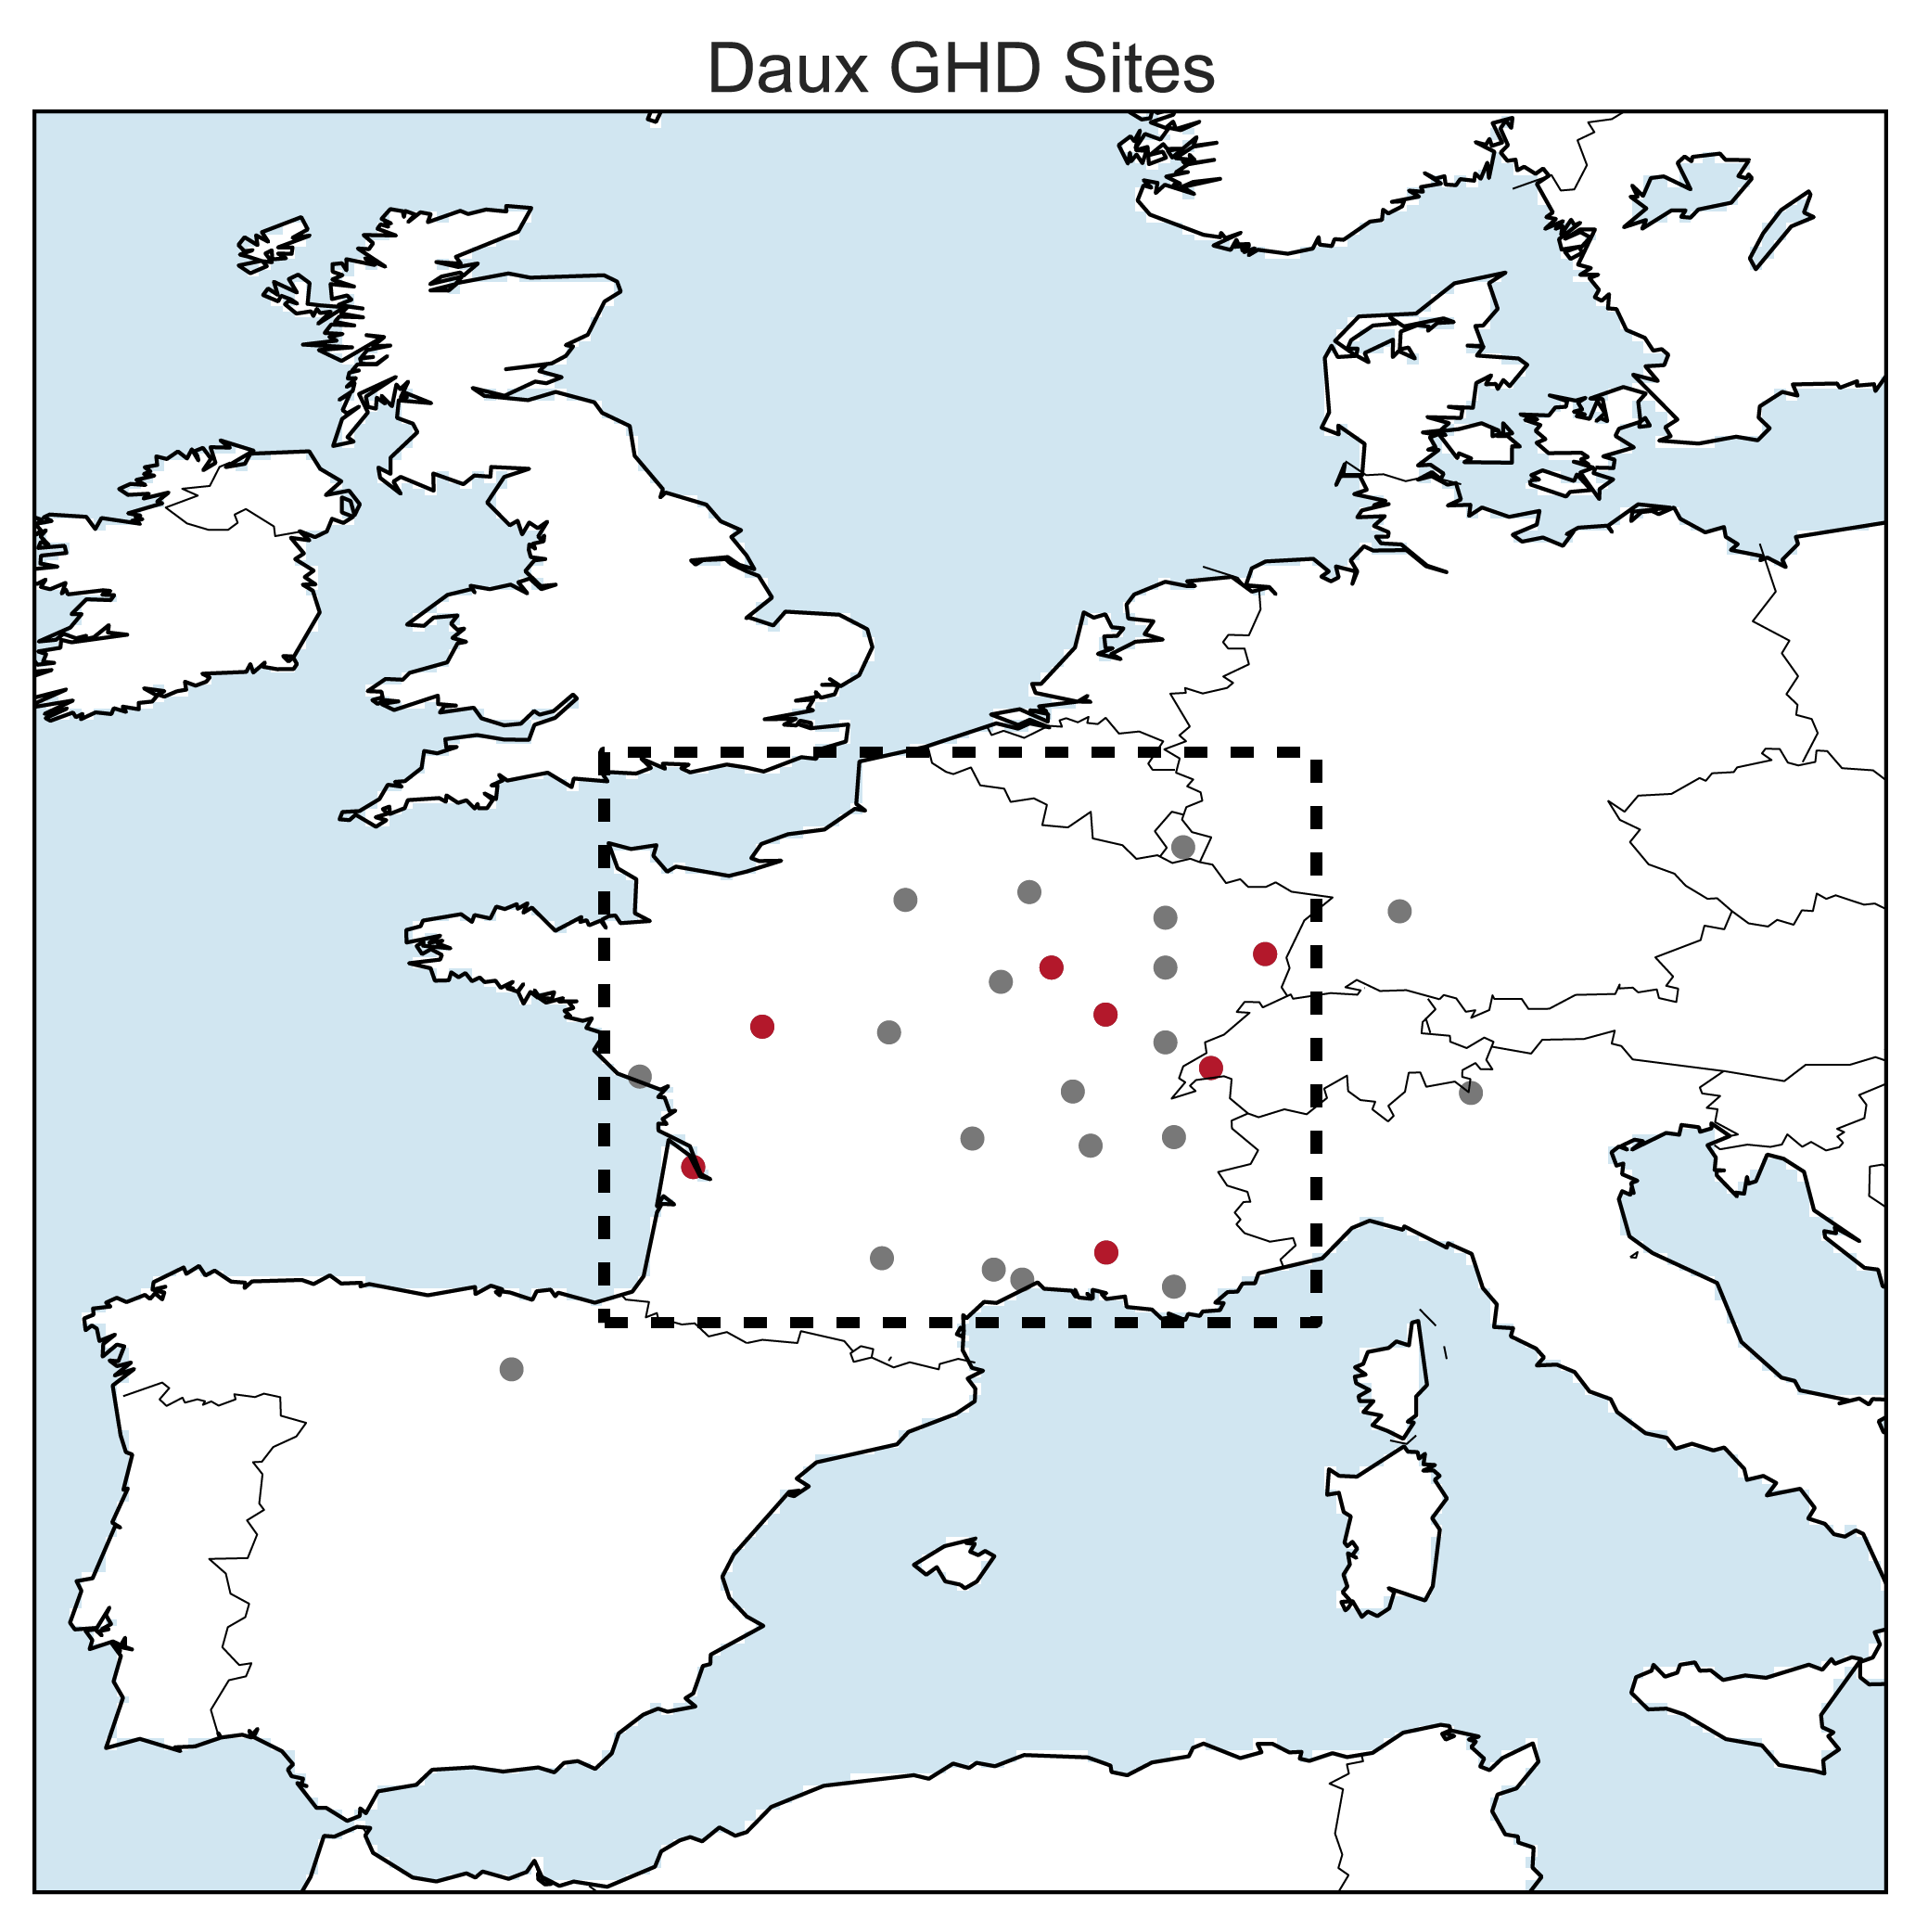
\includegraphics[width=1.0\columnwidth,scale=2]{SUPP_fig_01_map_sitelocs.png}
\caption{Geographic locations for all 27 regional GHD time series in DAUX. Highlighted in red are the sites that comprise the GHD-Core index: Alsace (Als), Bordeaux (Bor), Burgundy (Bur), Champagne 1 (Cha1), the Lower Loire Valley (LLV), the Southern Rhone Valley (SRv), and Switzerland at Lake Geneva (Swi). The dashed black box indicates the GHD-Core region (2\textsuperscript{o}W--8\textsuperscript{o}E, 43\textsuperscript{o}N--51\textsuperscript{o}N) over which climate anomalies from the CRU instrumental climate datasets and the three reconstructions were averaged for the various regression analyses.}
\end{figure}

\begin{figure}
\center
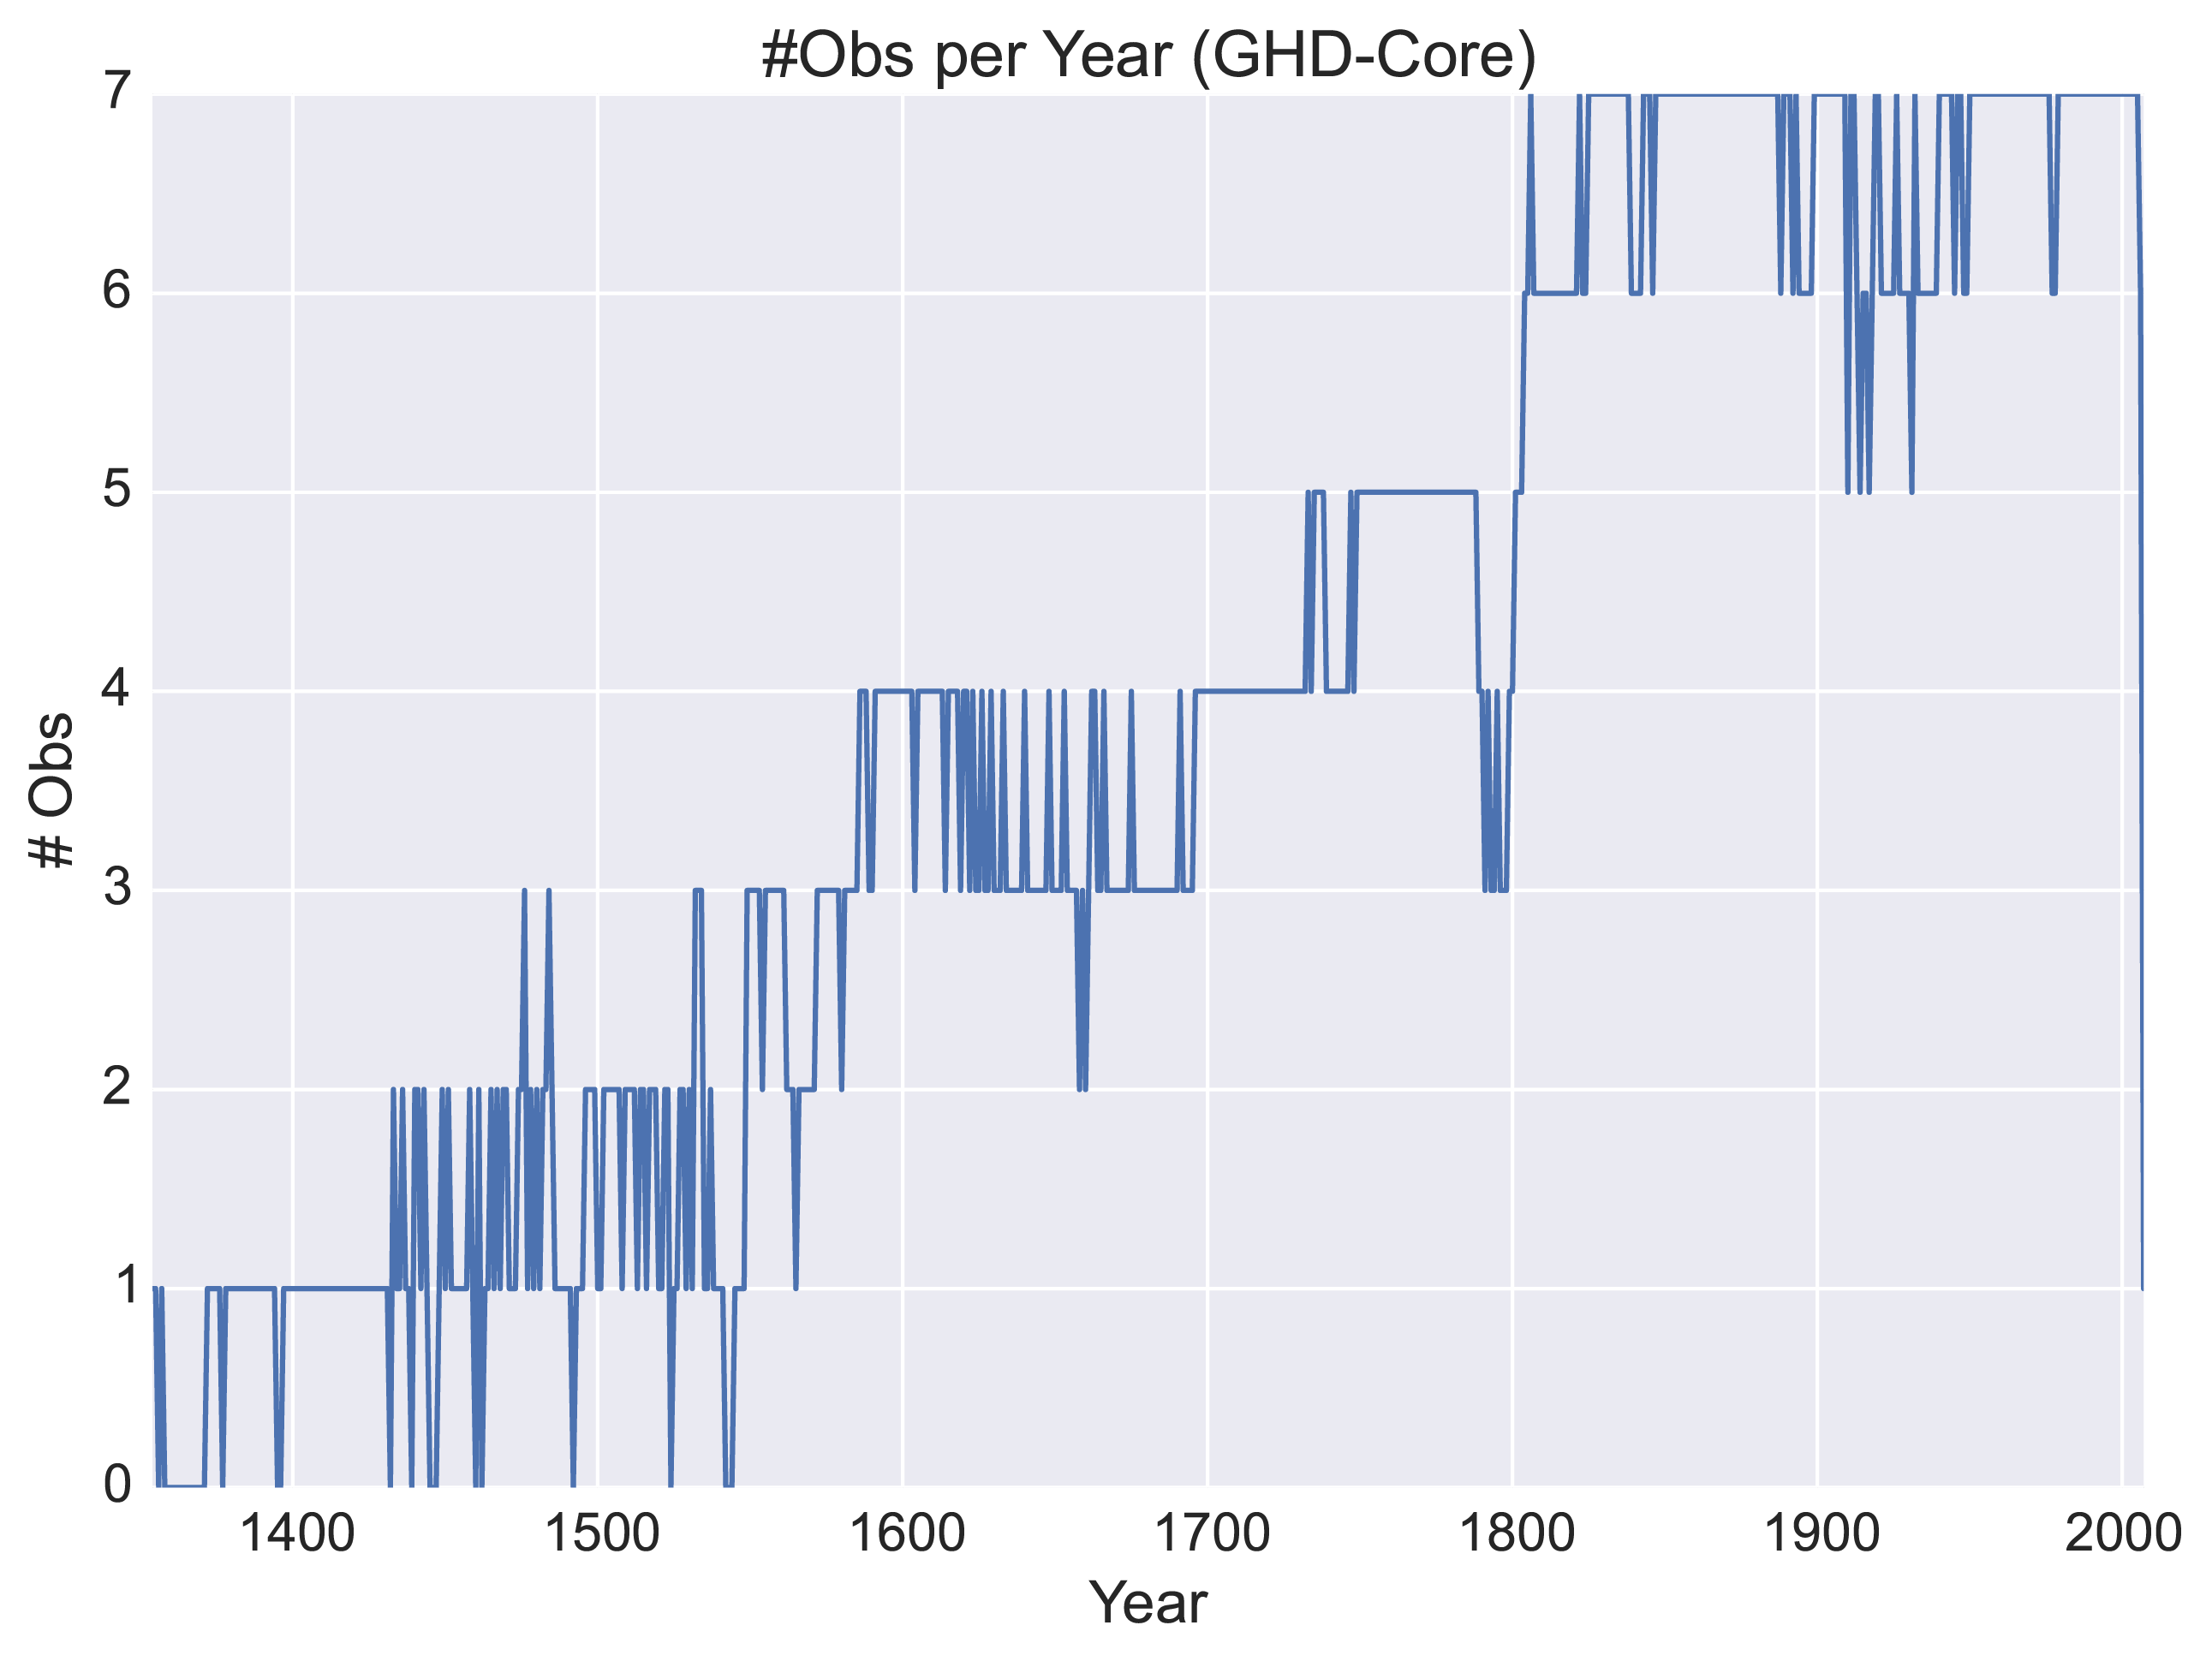
\includegraphics[width=1.0\columnwidth,scale=2]{SUPP_fig_02_numobs.png}
\caption{Number of observations (i.e., regional GHD series) represented in each year of the GHD-Core index.}
\end{figure}

\begin{sidewaysfigure}
\center
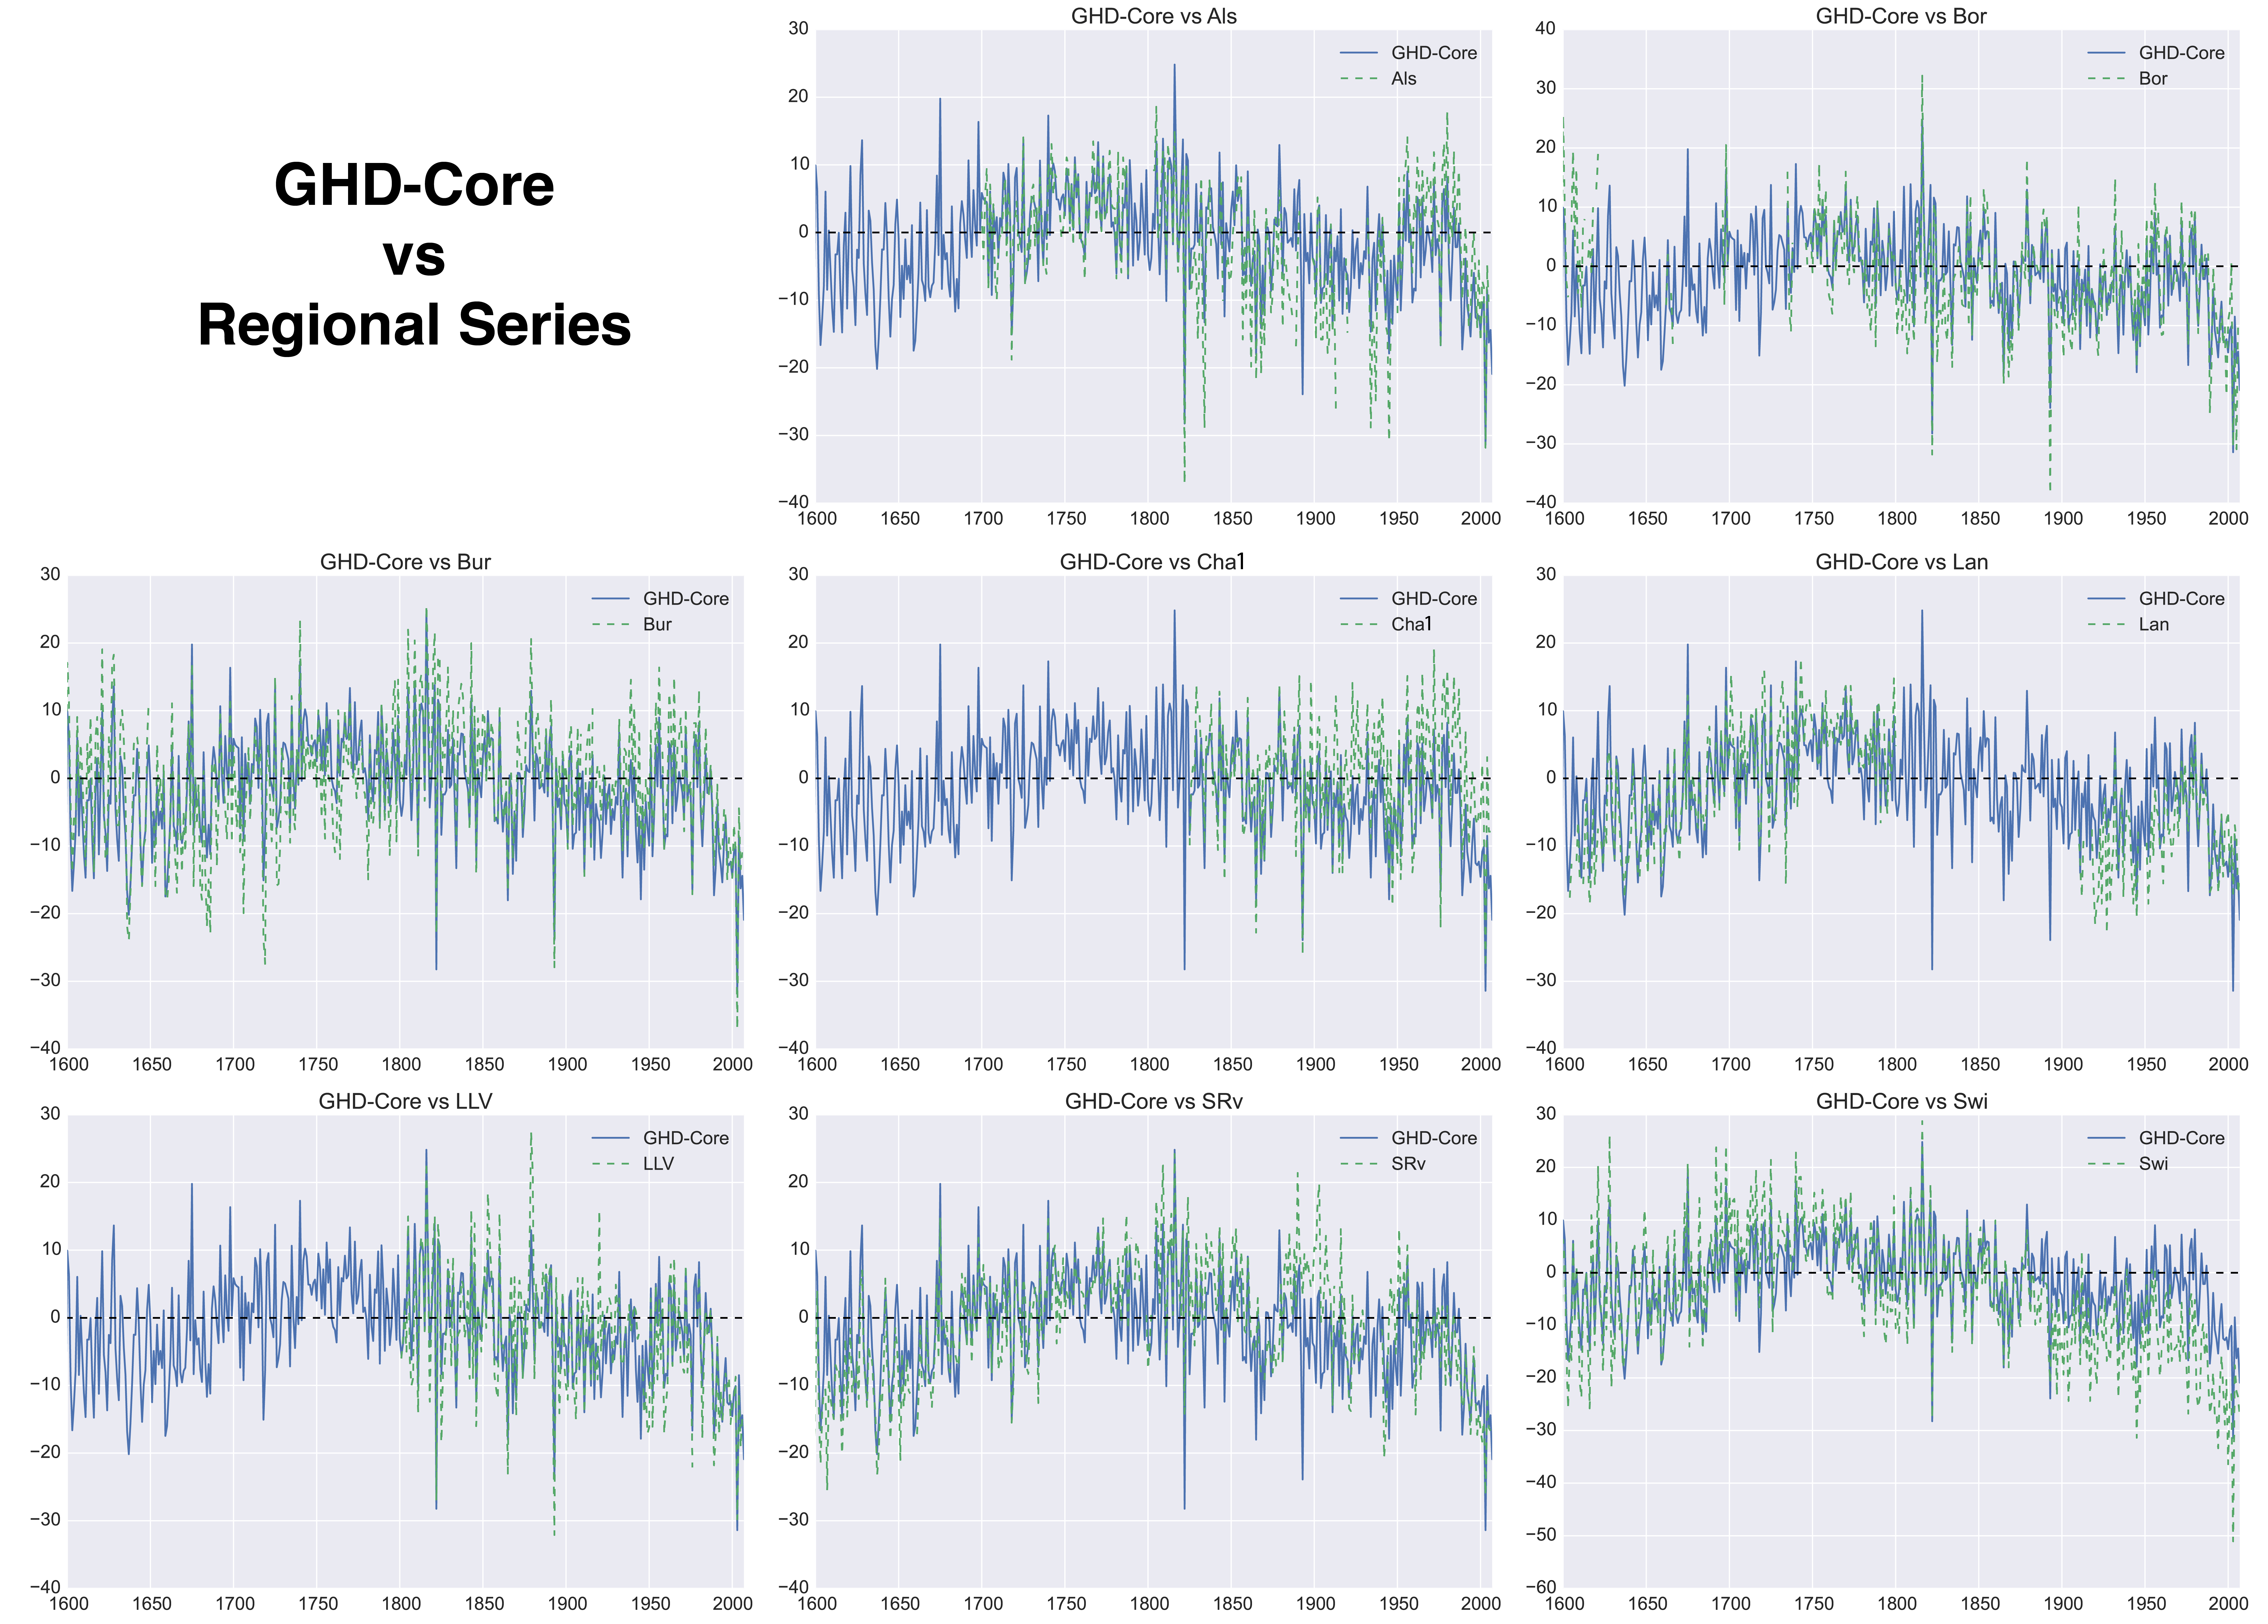
\includegraphics[width=1.0\columnwidth,scale=2]{SUPP_fig_03_core_vs_sites.png}
\caption{Time series (1600--2007) of GHD-Core (blue sold line) and each individual regional GHD series (green dashed lines).}
\end{sidewaysfigure}

\begin{figure}
\center
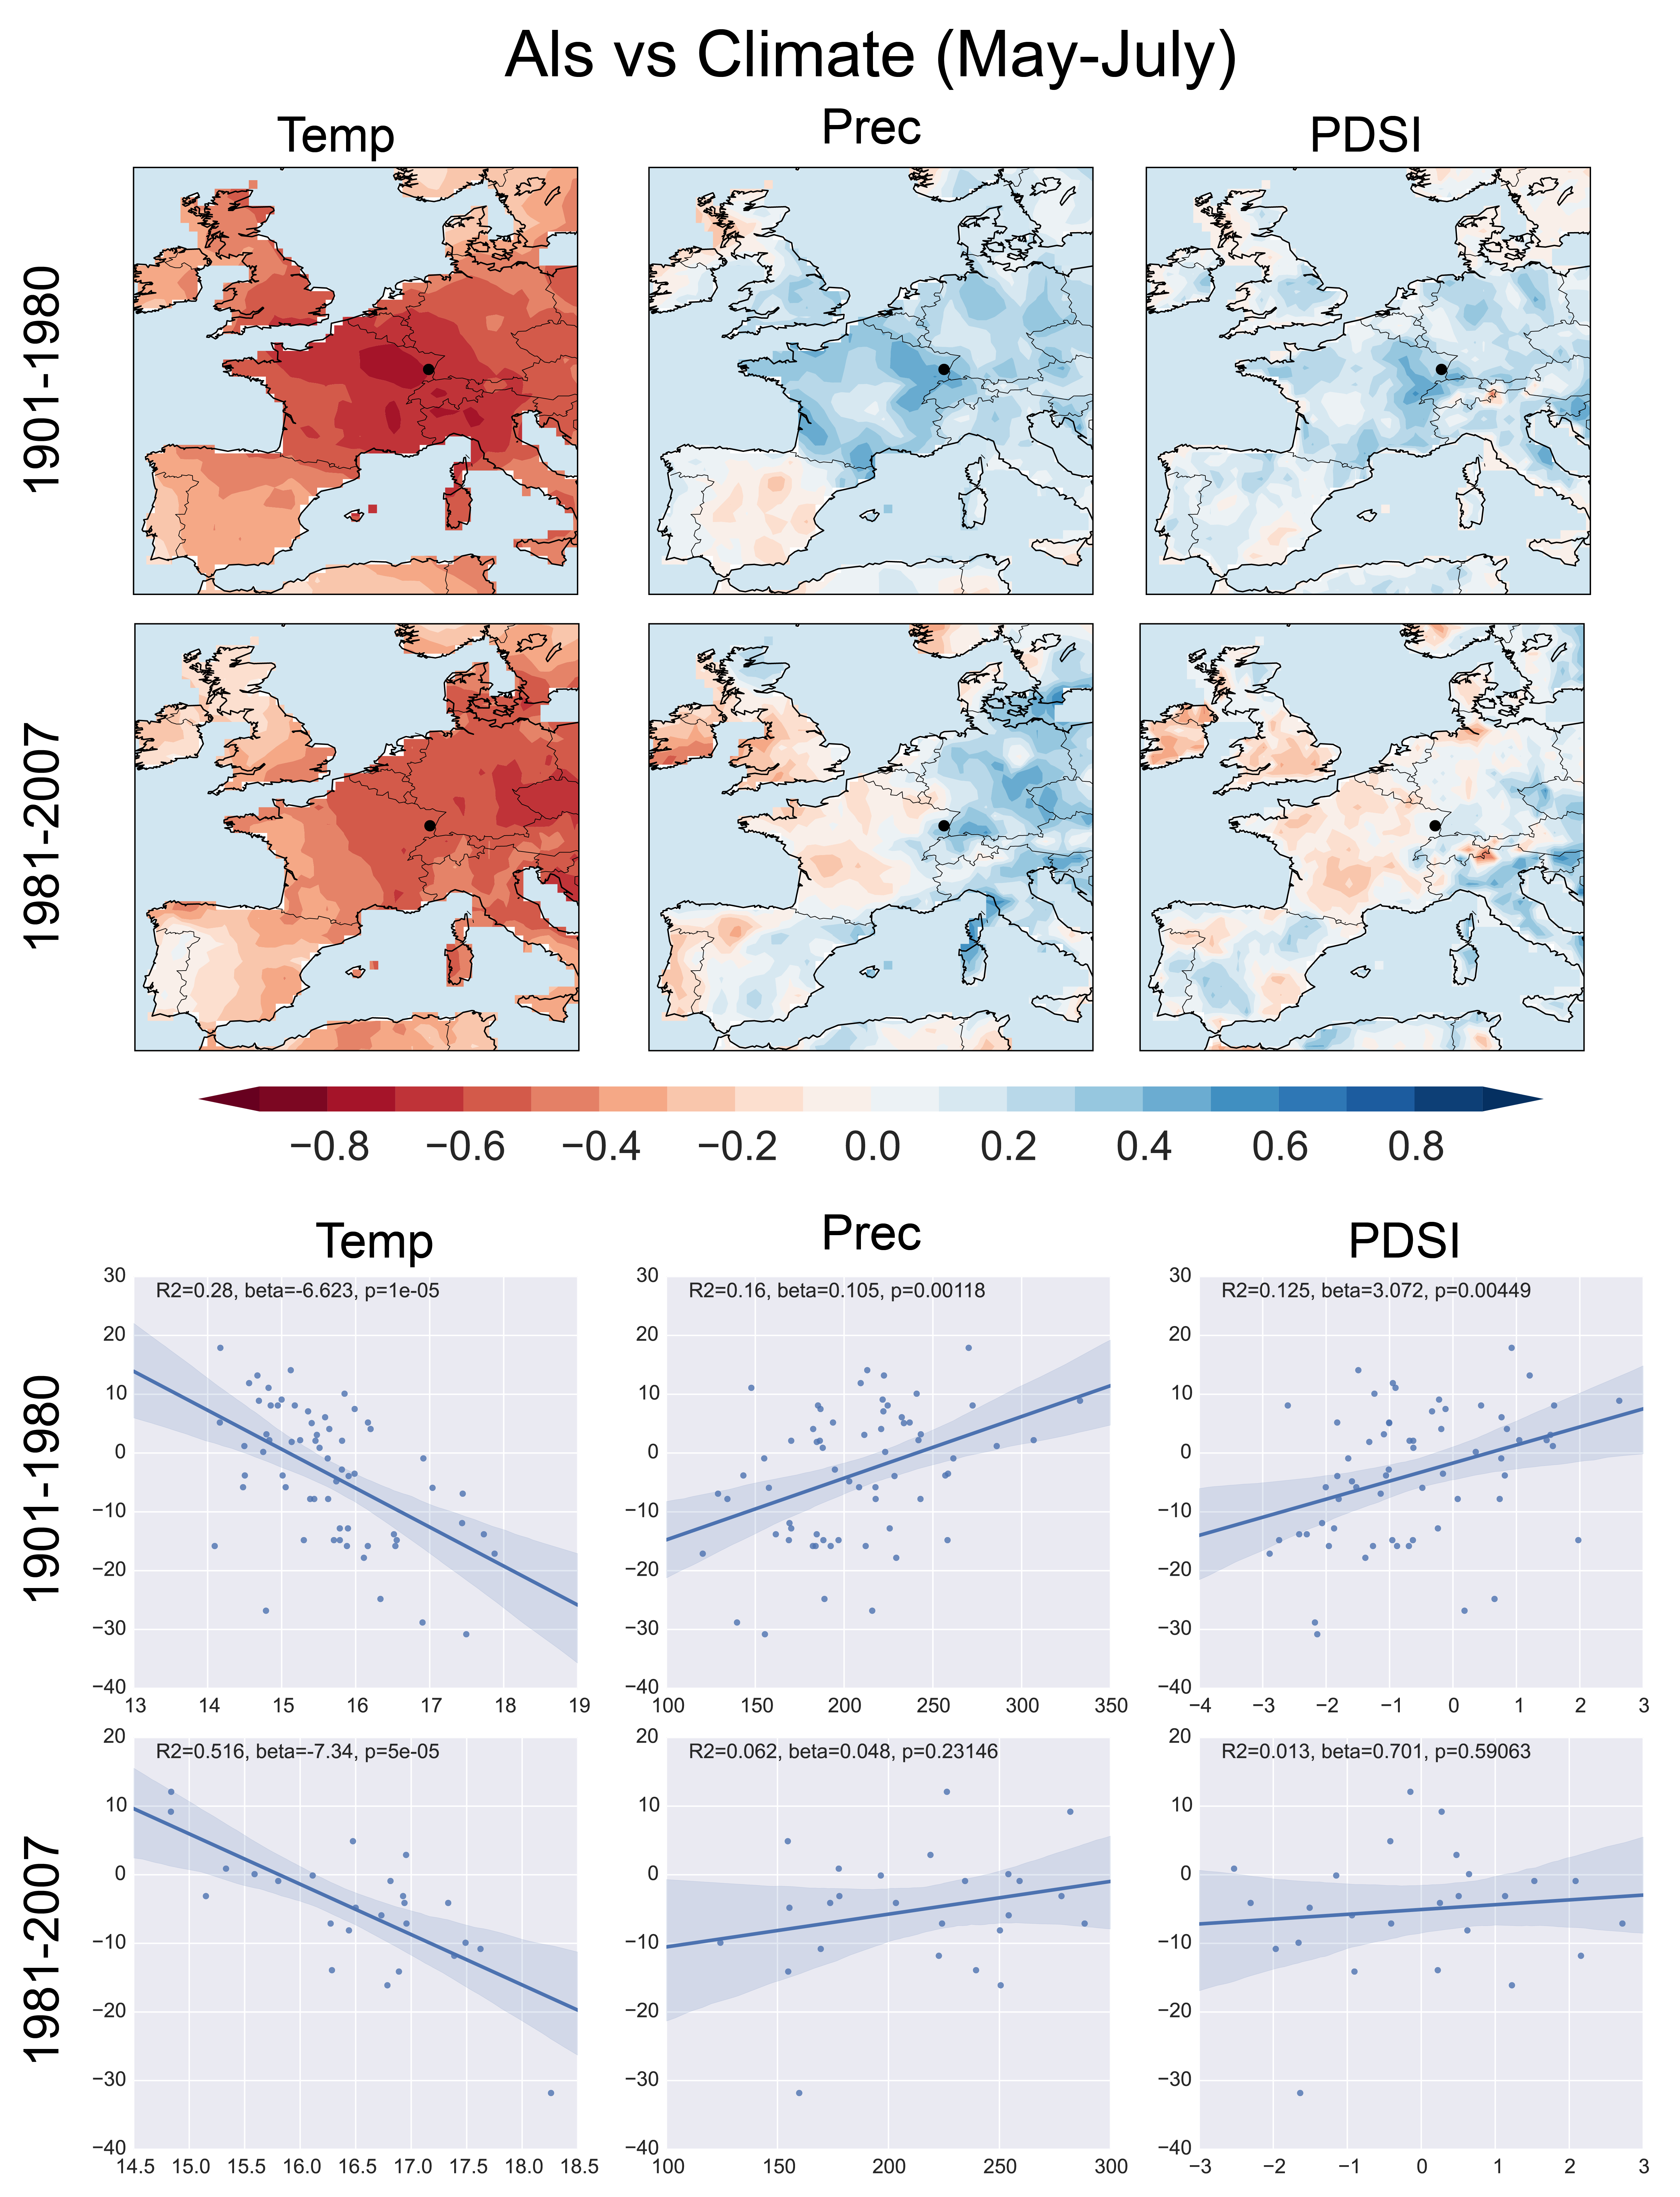
\includegraphics[width=.9\columnwidth,scale=2]{SUPP_fig_04_ALS_MJJ_climate.png}
\caption{Comparisons between the GHD series from ALS and May-June-July temperature, precipitation, and PDSI from the CRU 3.21 climate grids. Top panels: point-by-point correlations for 1901--1980 and 1981--2007 (location of ALS is shown by the black dot). Bottom panels: linear regression plots for the same intervals against CRU climate data averaged within one degree of the site location.}
\end{figure}

\begin{figure}
\center
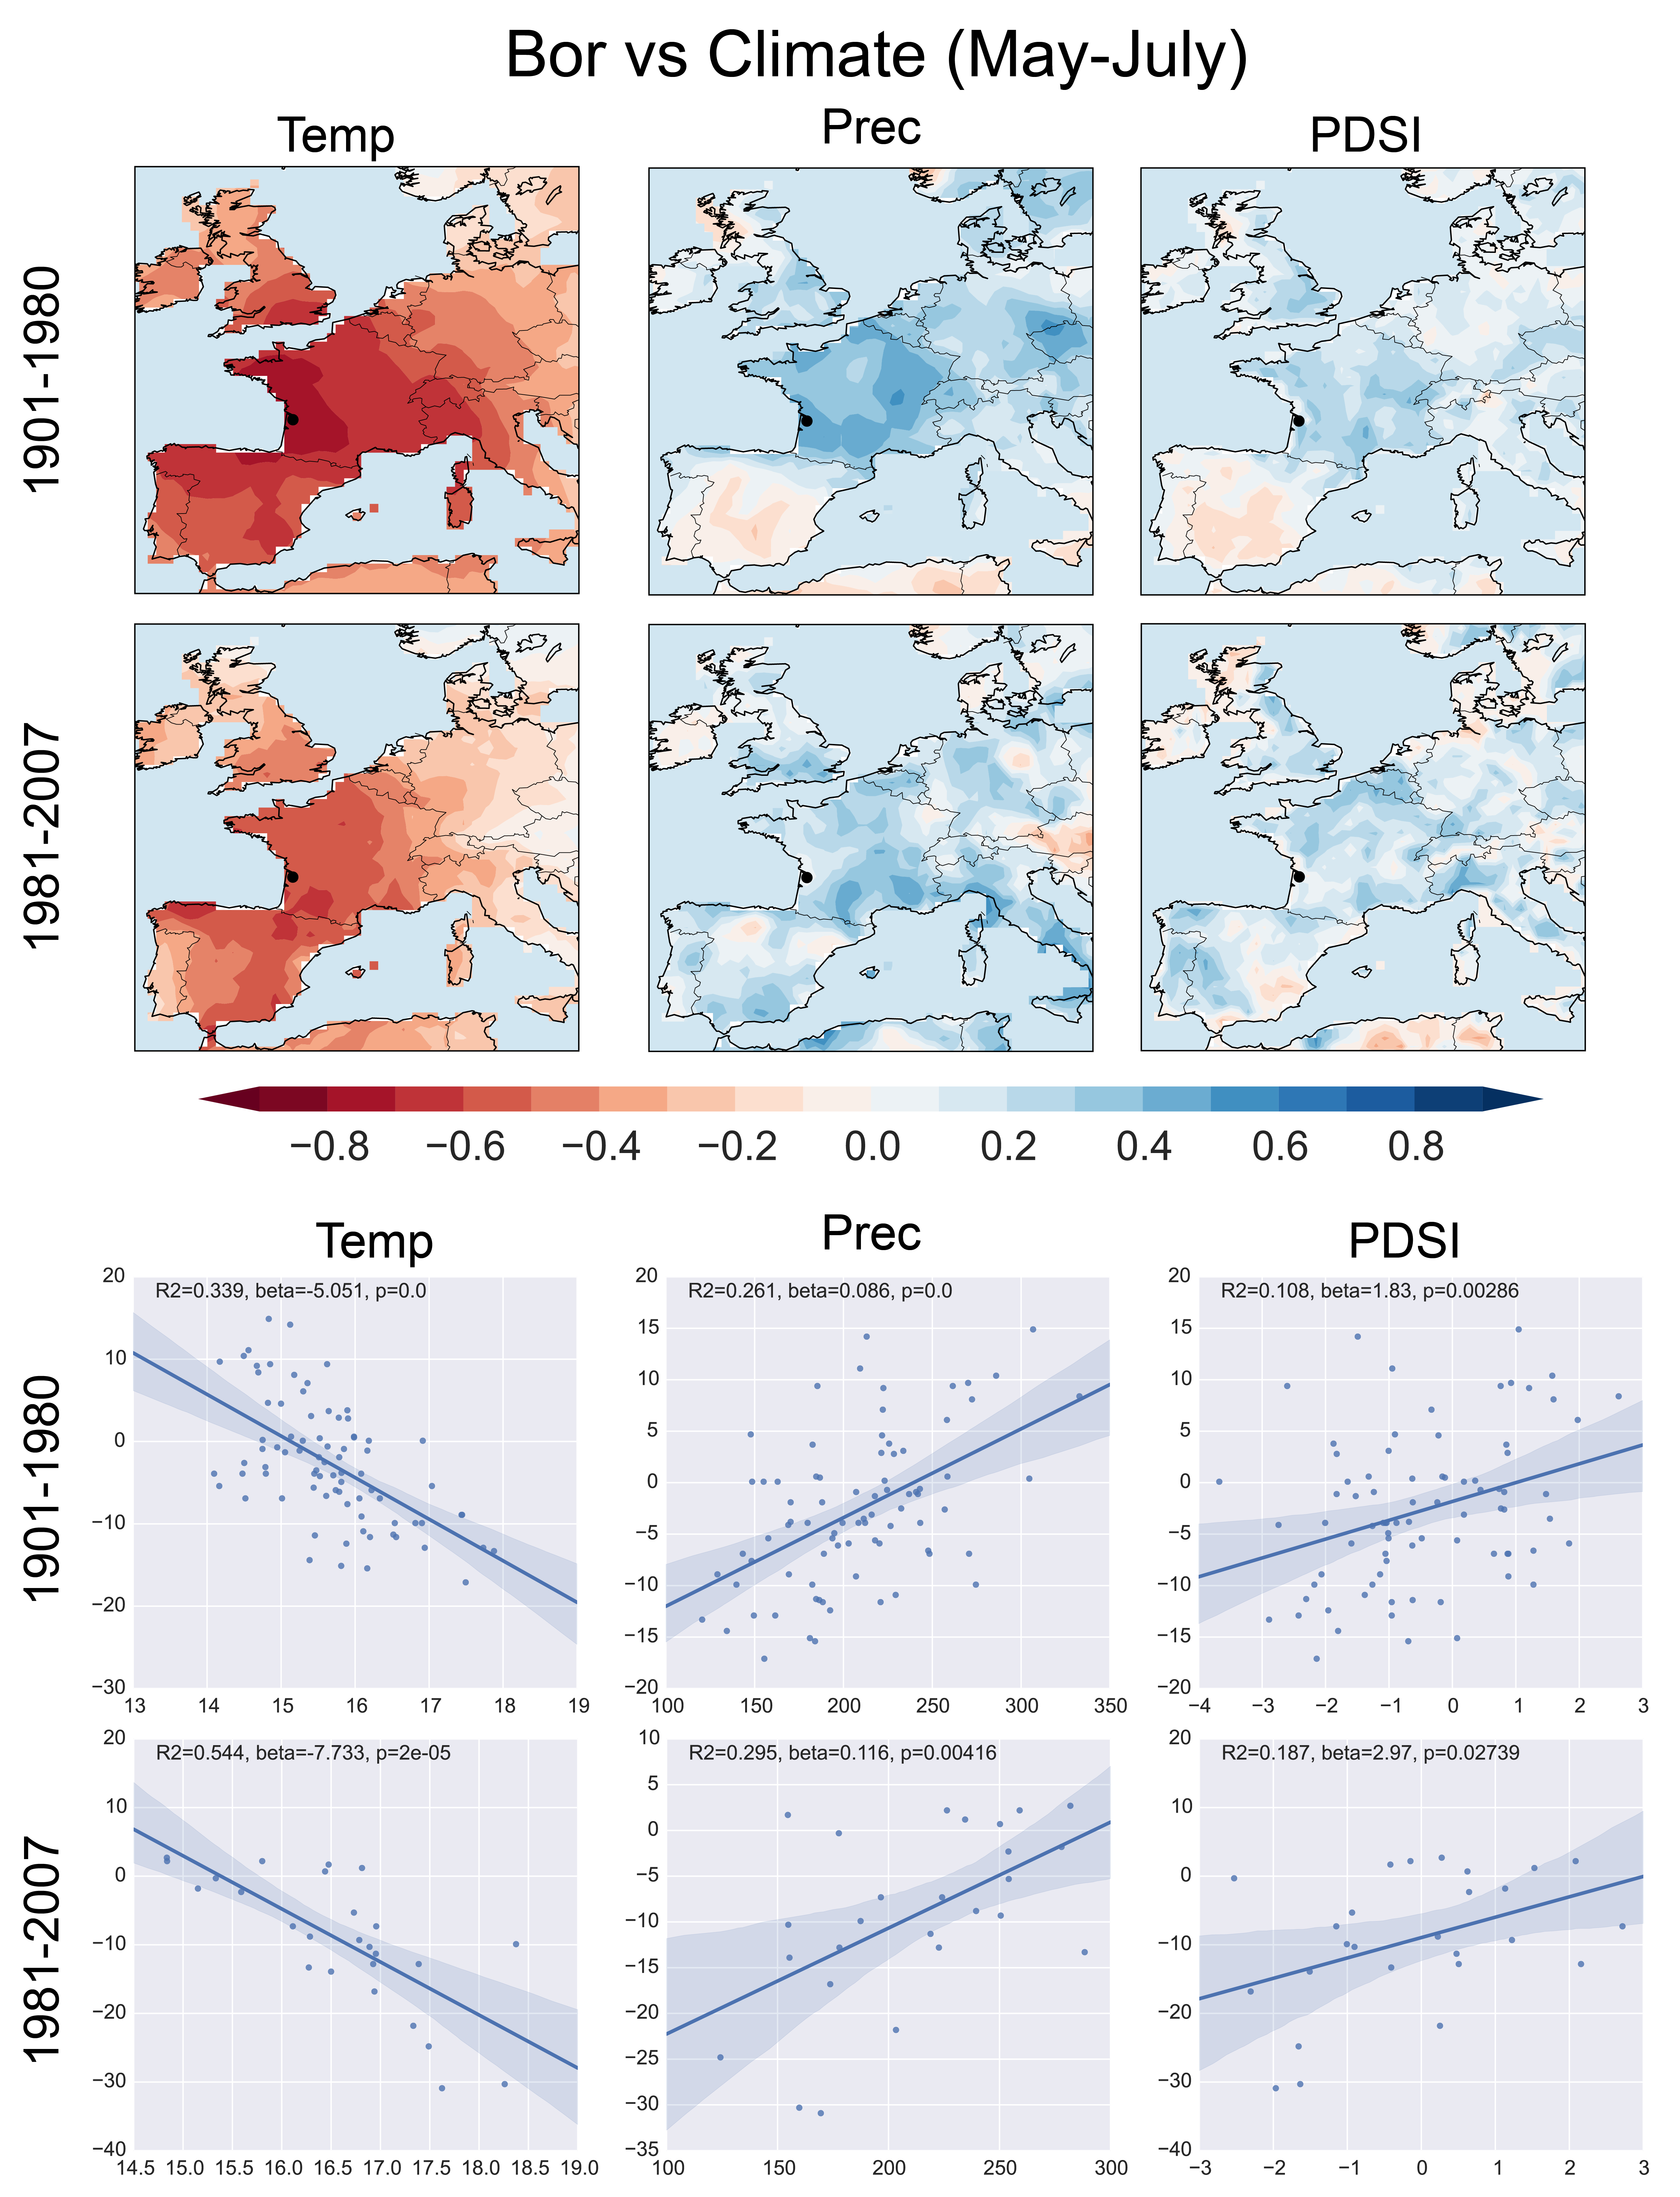
\includegraphics[width=.9\columnwidth,scale=2]{SUPP_fig_05_Bor_MJJ_climate.png}
\caption{Same as Figure 4, but for Bor.}
\end{figure}

\begin{figure}
\center
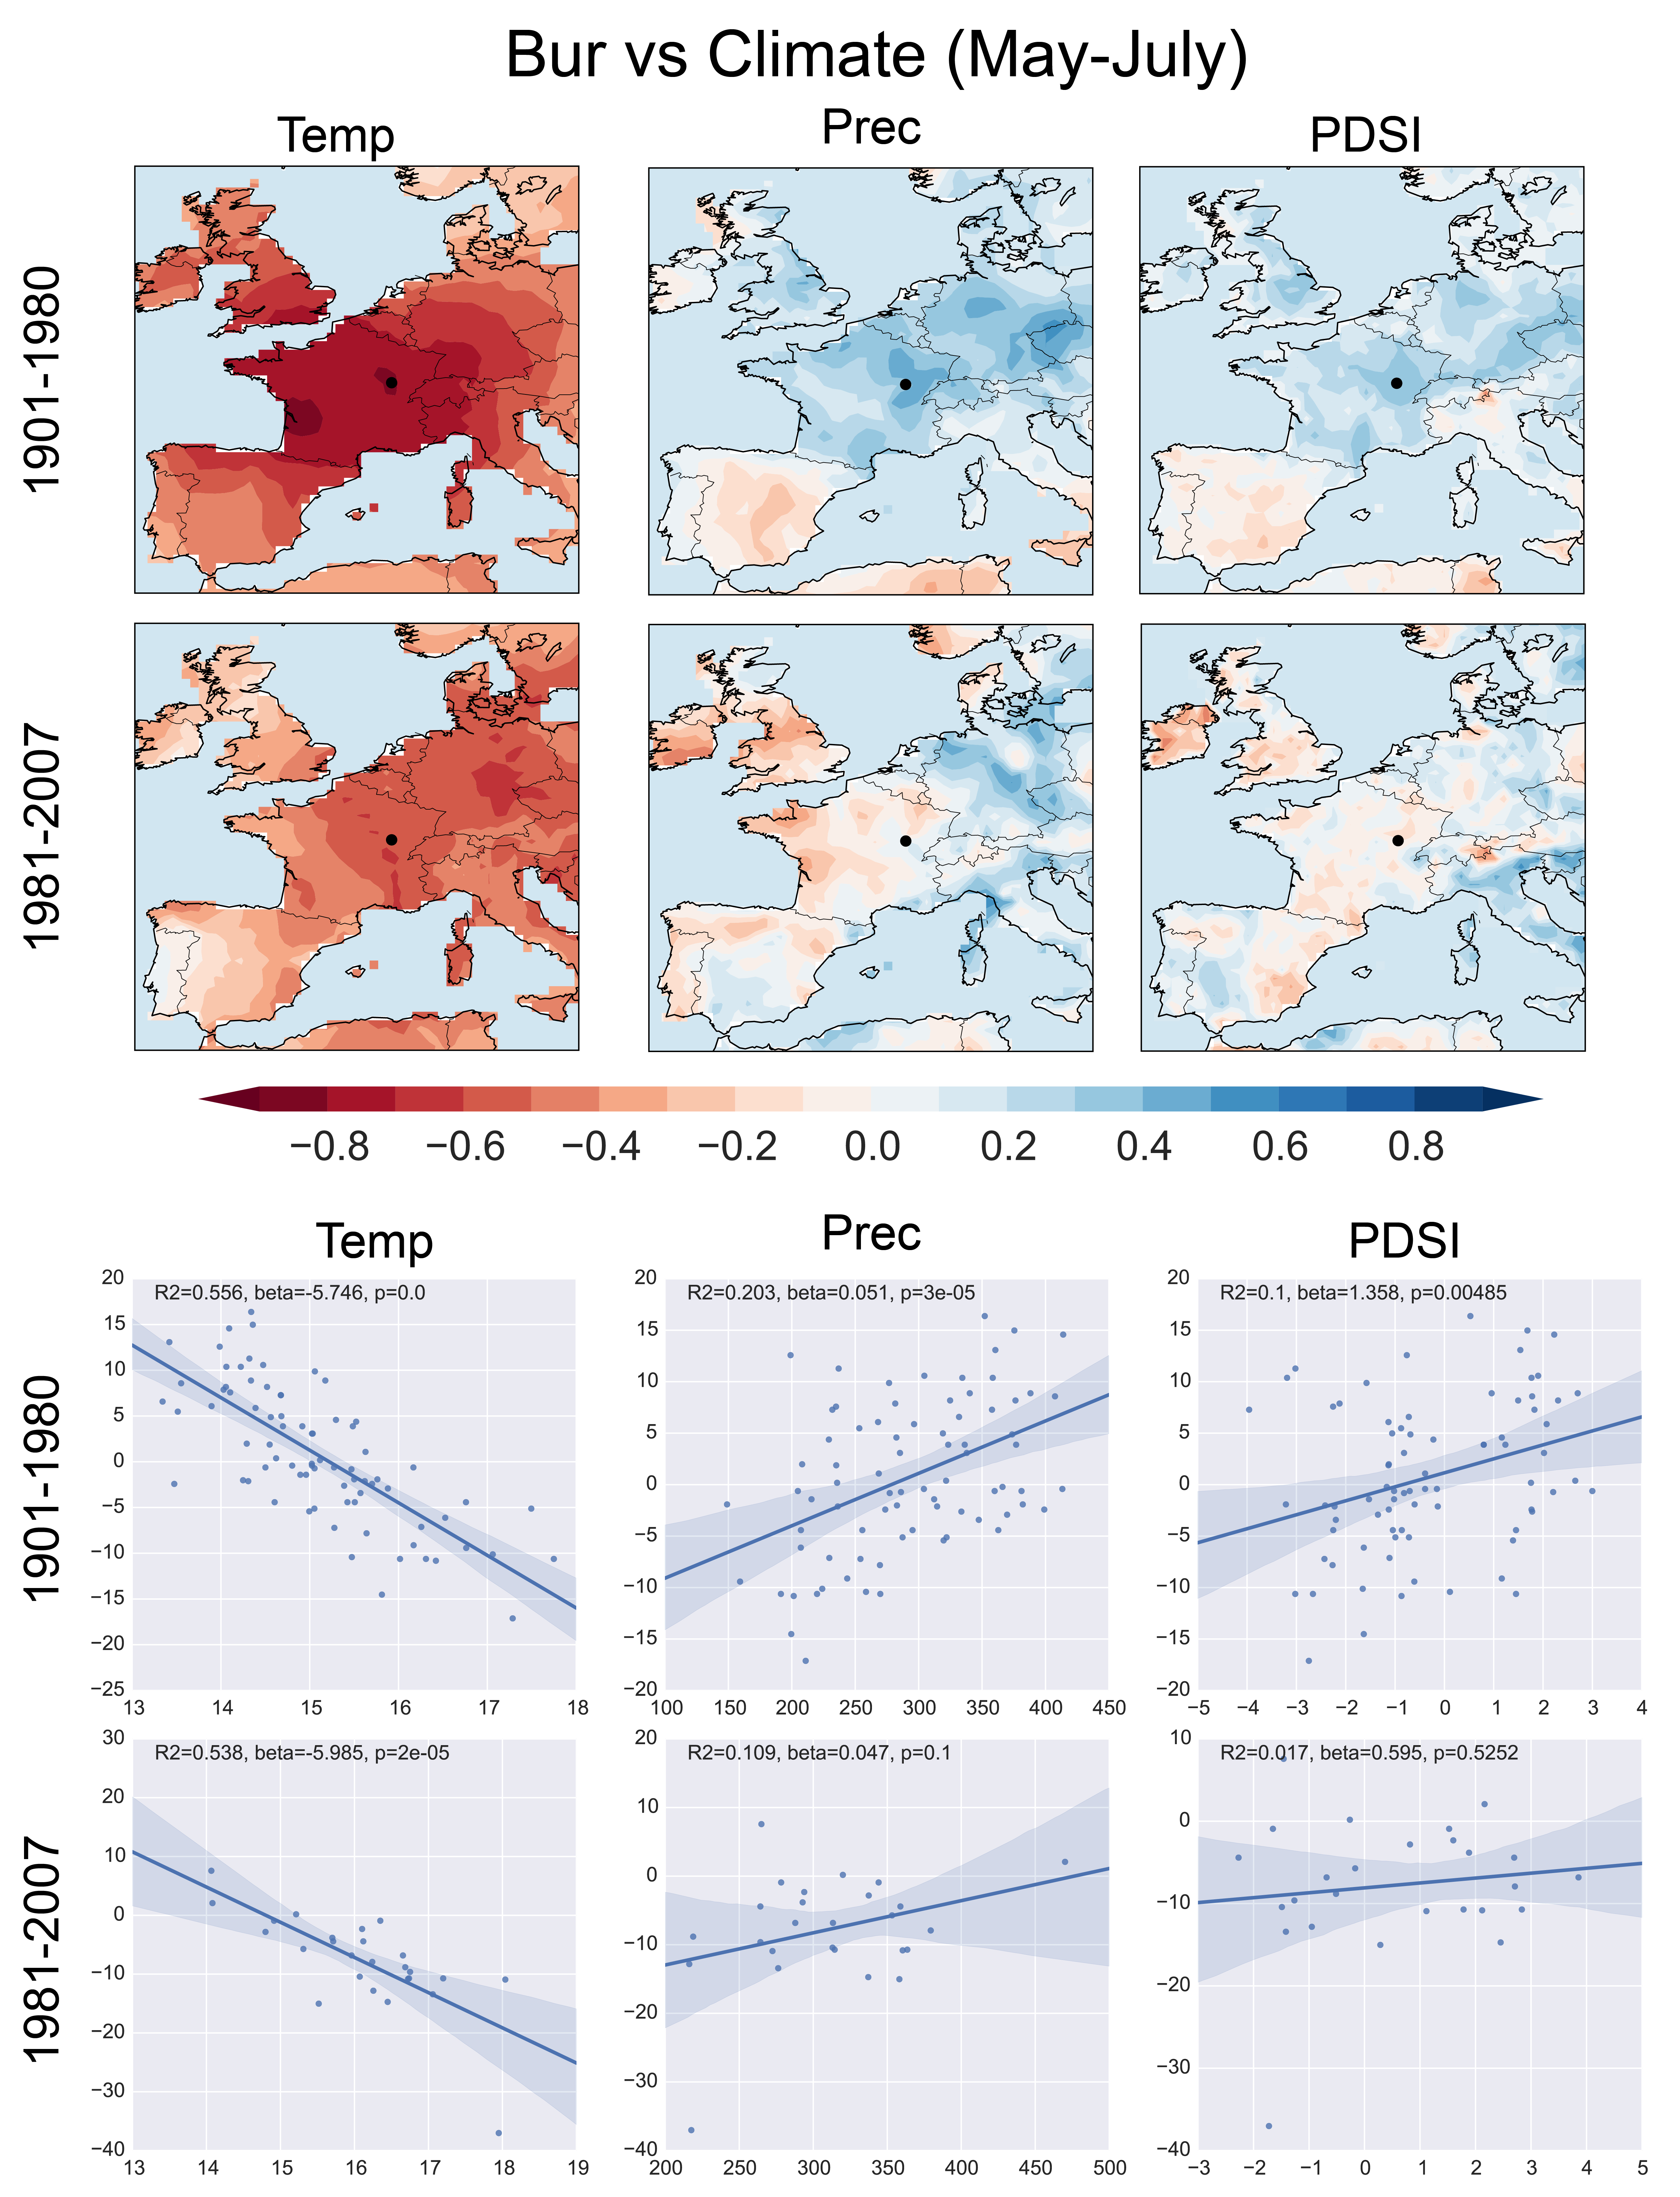
\includegraphics[width=.9\columnwidth,scale=2]{SUPP_fig_06_Bur_MJJ_climate.png}
\caption{Same as Figure 4, but for Bur.}
\end{figure}

\begin{figure}
\center
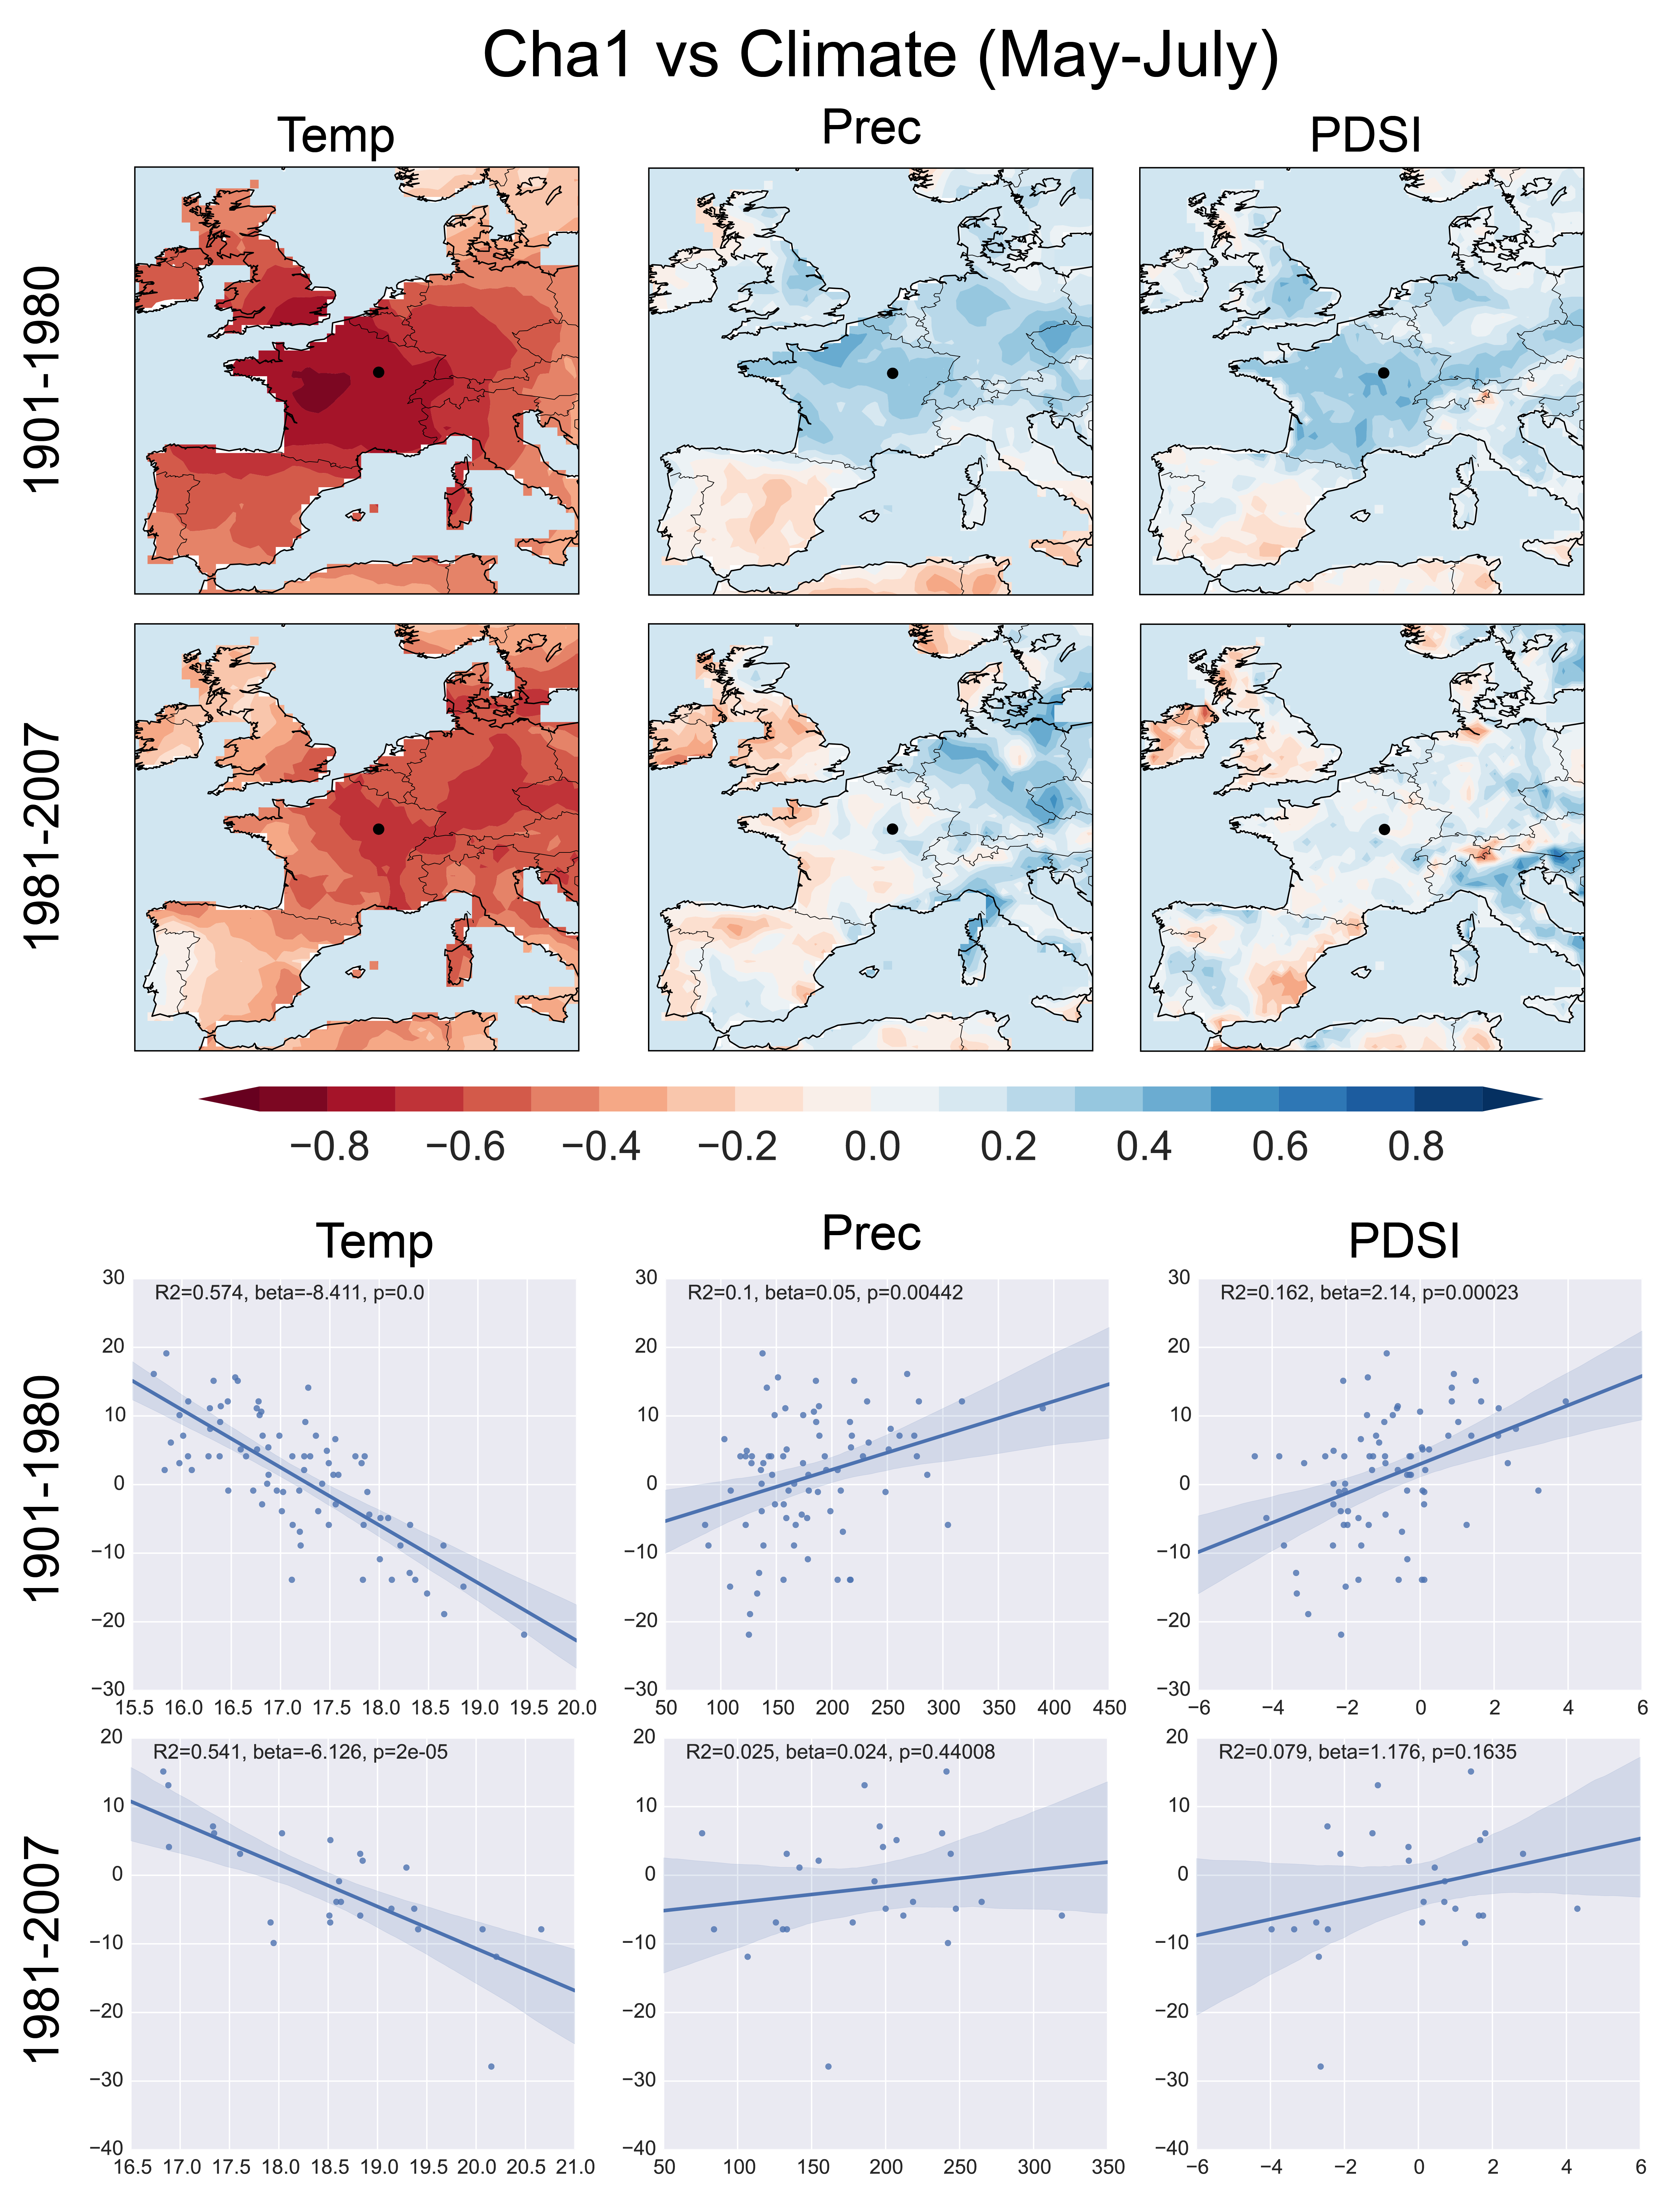
\includegraphics[width=.9\columnwidth,scale=2]{SUPP_fig_07_Cha1_MJJ_climate.png}
\caption{Same as Figure 4, but for Cha1.}
\end{figure}

\begin{figure}
\center
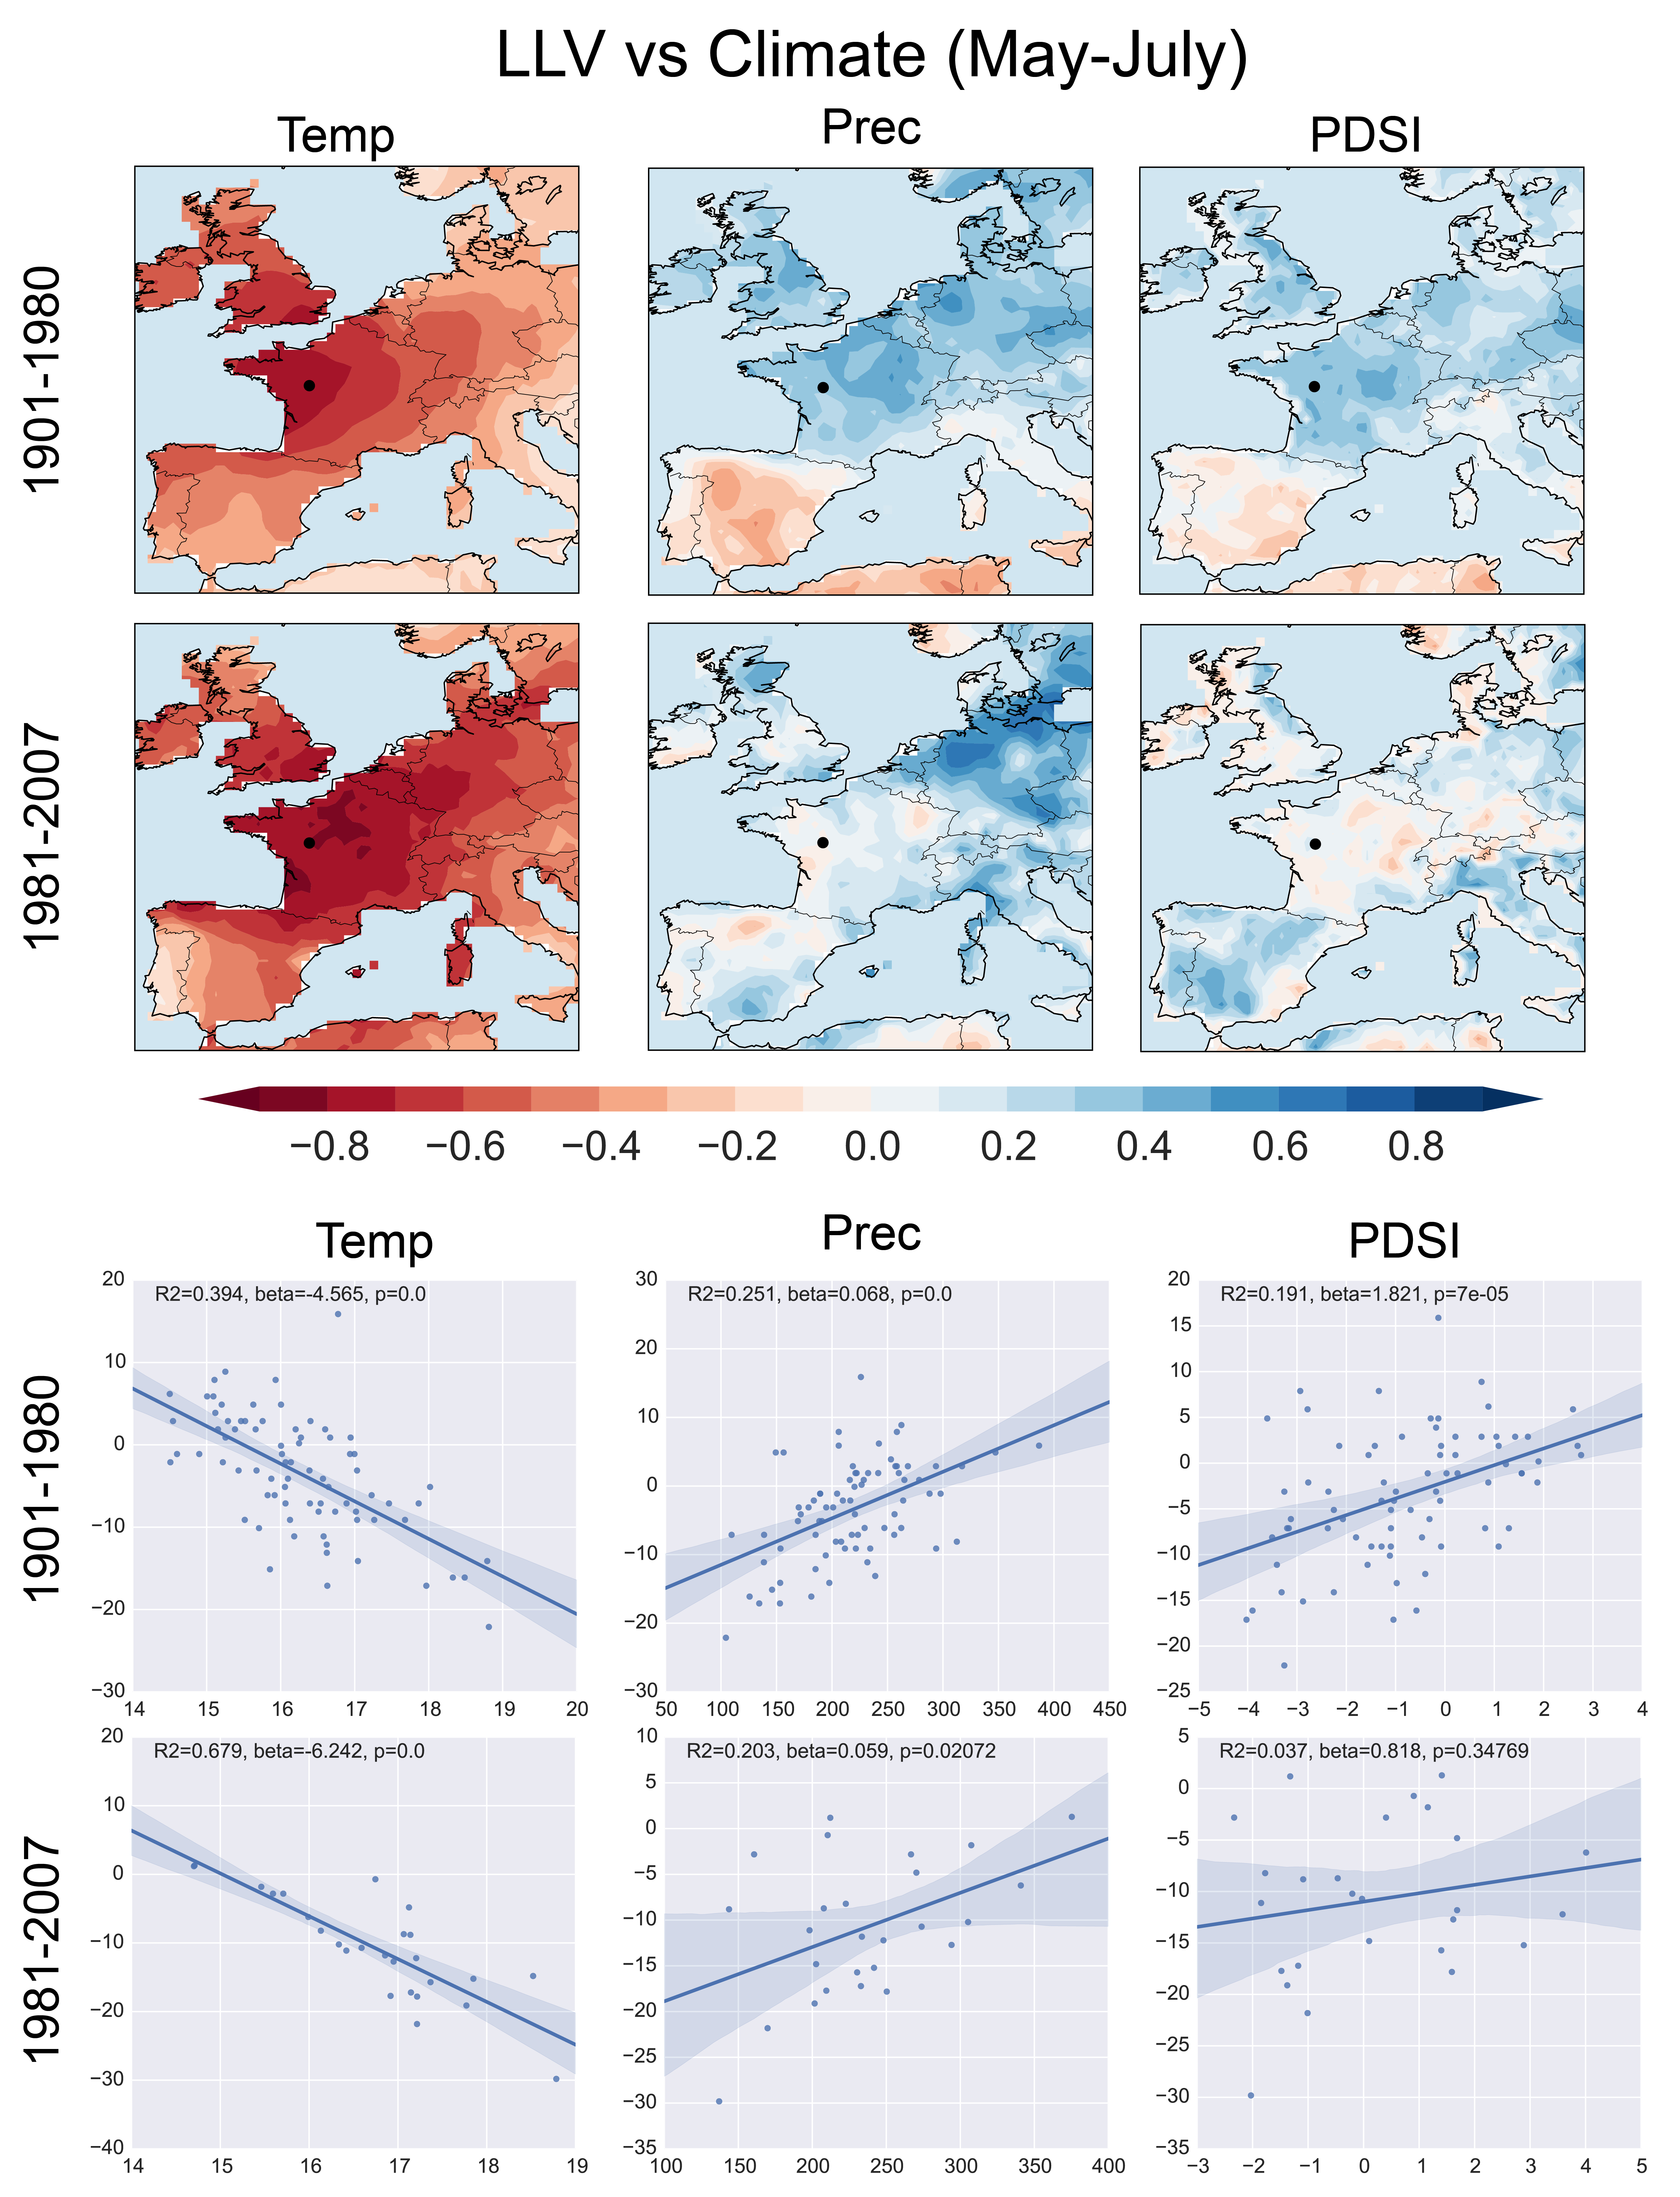
\includegraphics[width=.9\columnwidth,scale=2]{SUPP_fig_08_LLV_MJJ_climate.png}
\caption{Same as Figure 4, but for LLV.}
\end{figure}

\begin{figure}
\center
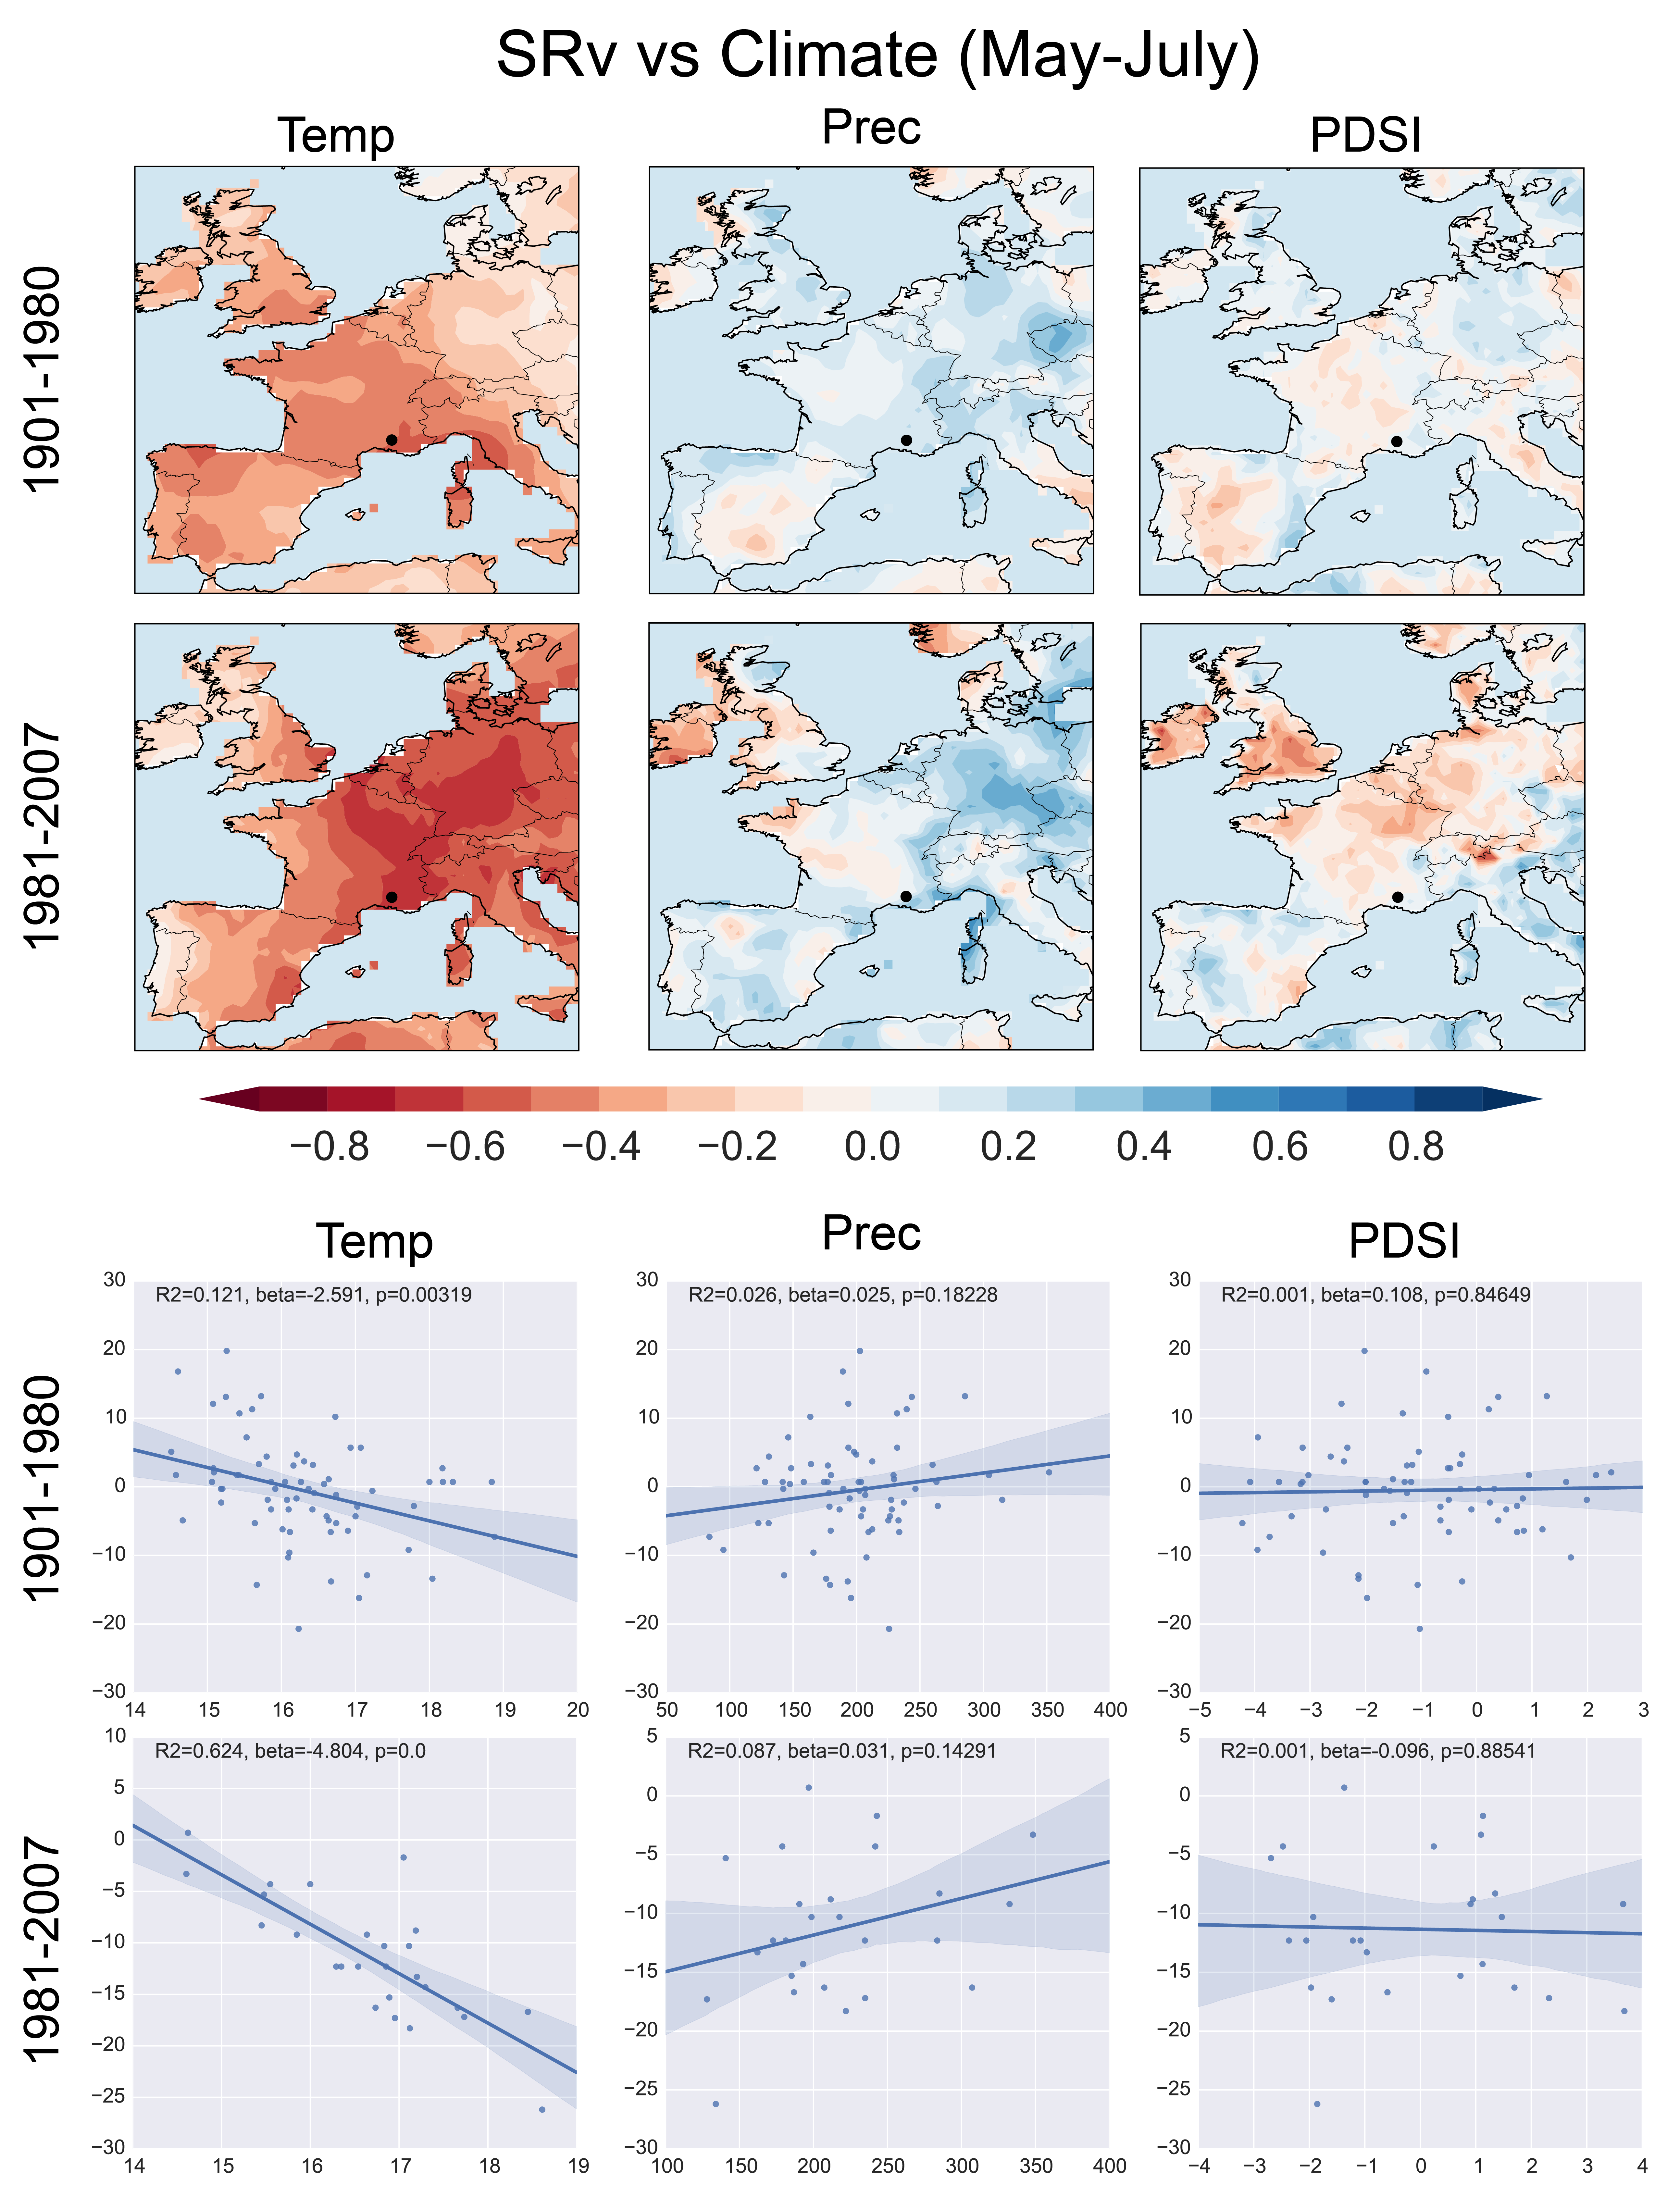
\includegraphics[width=.9\columnwidth,scale=2]{SUPP_fig_09_SRv_MJJ_climate.png}
\caption{Same as Figure 4, but for SRv.}
\end{figure}

\begin{figure}
\center
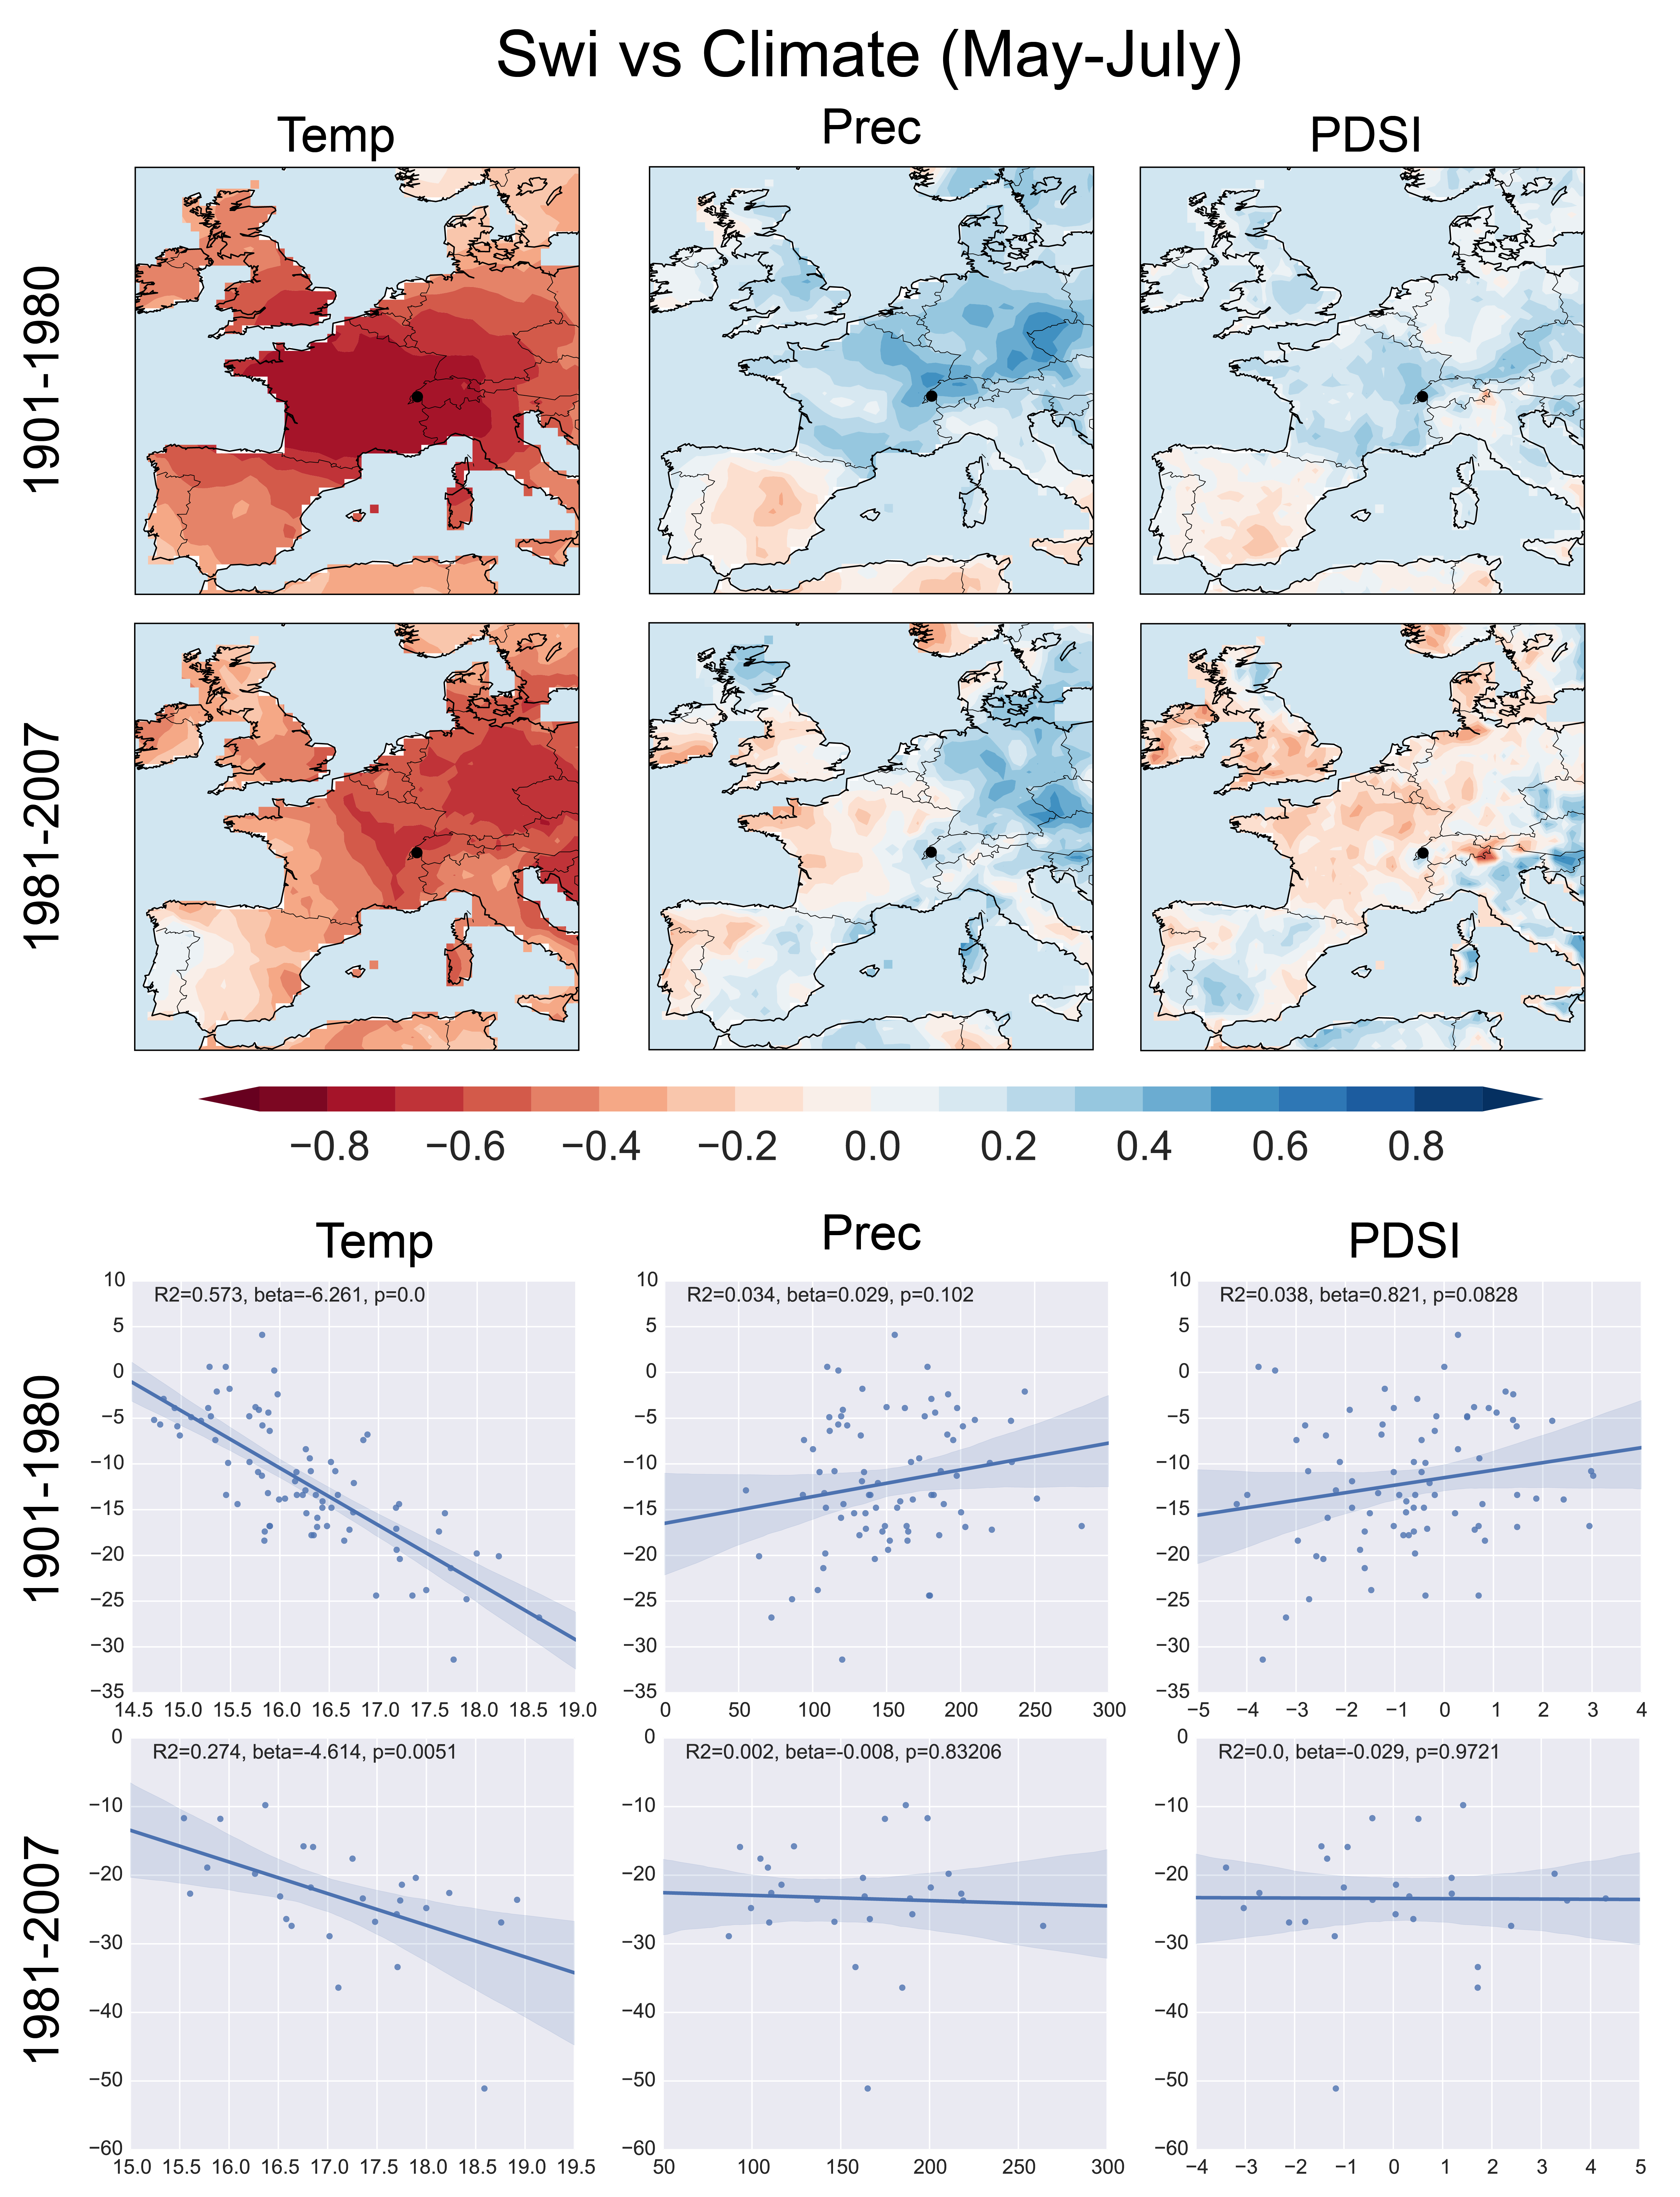
\includegraphics[width=.9\columnwidth,scale=2]{SUPP_fig_10_SWi_MJJ_climate.png}
\caption{Same as Figure 4, but for SWi.}
\end{figure}

\begin{figure}
\center
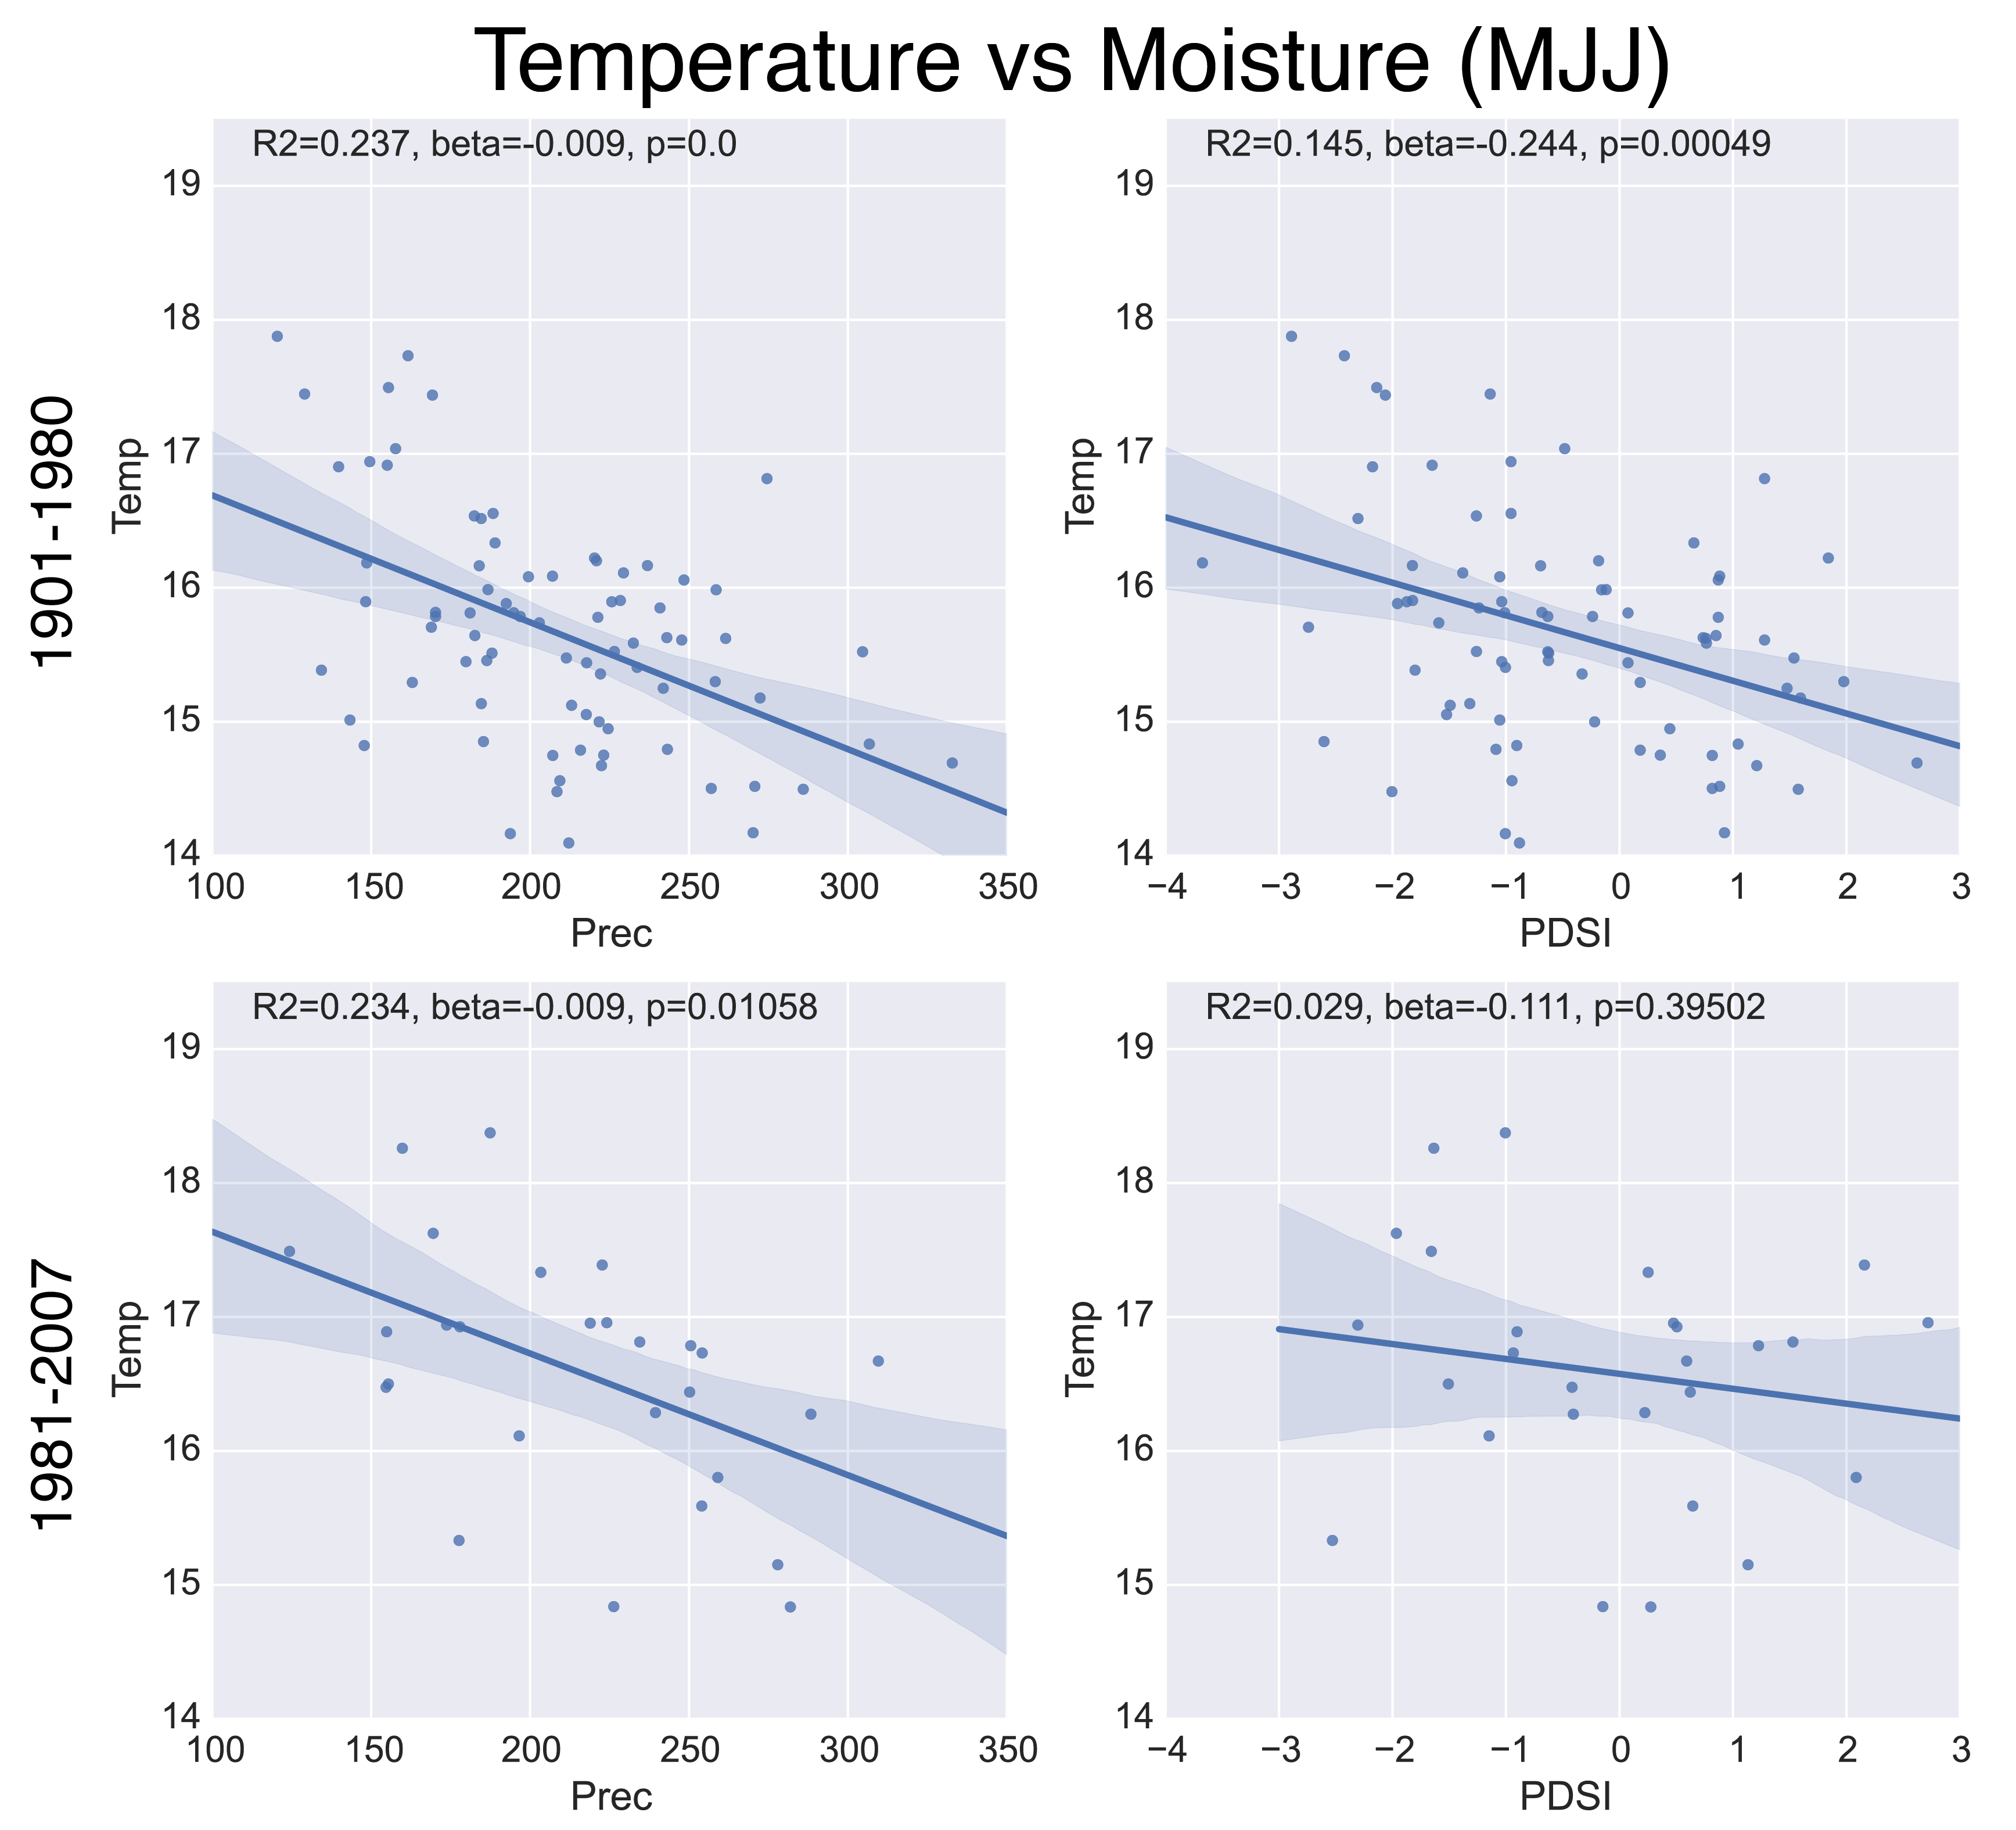
\includegraphics[width=1.0\columnwidth,scale=2]{SUPP_fig_11_temp_vs_moist_MJJ.png}
\caption{Temperature versus moisture (precipitation and PDSI) during May-June-July for the GHD-Core region from the CRU 3.21 climate grids for two periods: 1901--1980 and 1981--2007. Temperature during MJJ has a significant negative relationship with both precipitation and PDSI, indicating the tendency for warmer conditions during drier years. Over the more recent period, the relationship between temperature and PDSI breaks down, but the relationship with precipitation remains largely consistent.}
\end{figure}

\begin{figure}
\center
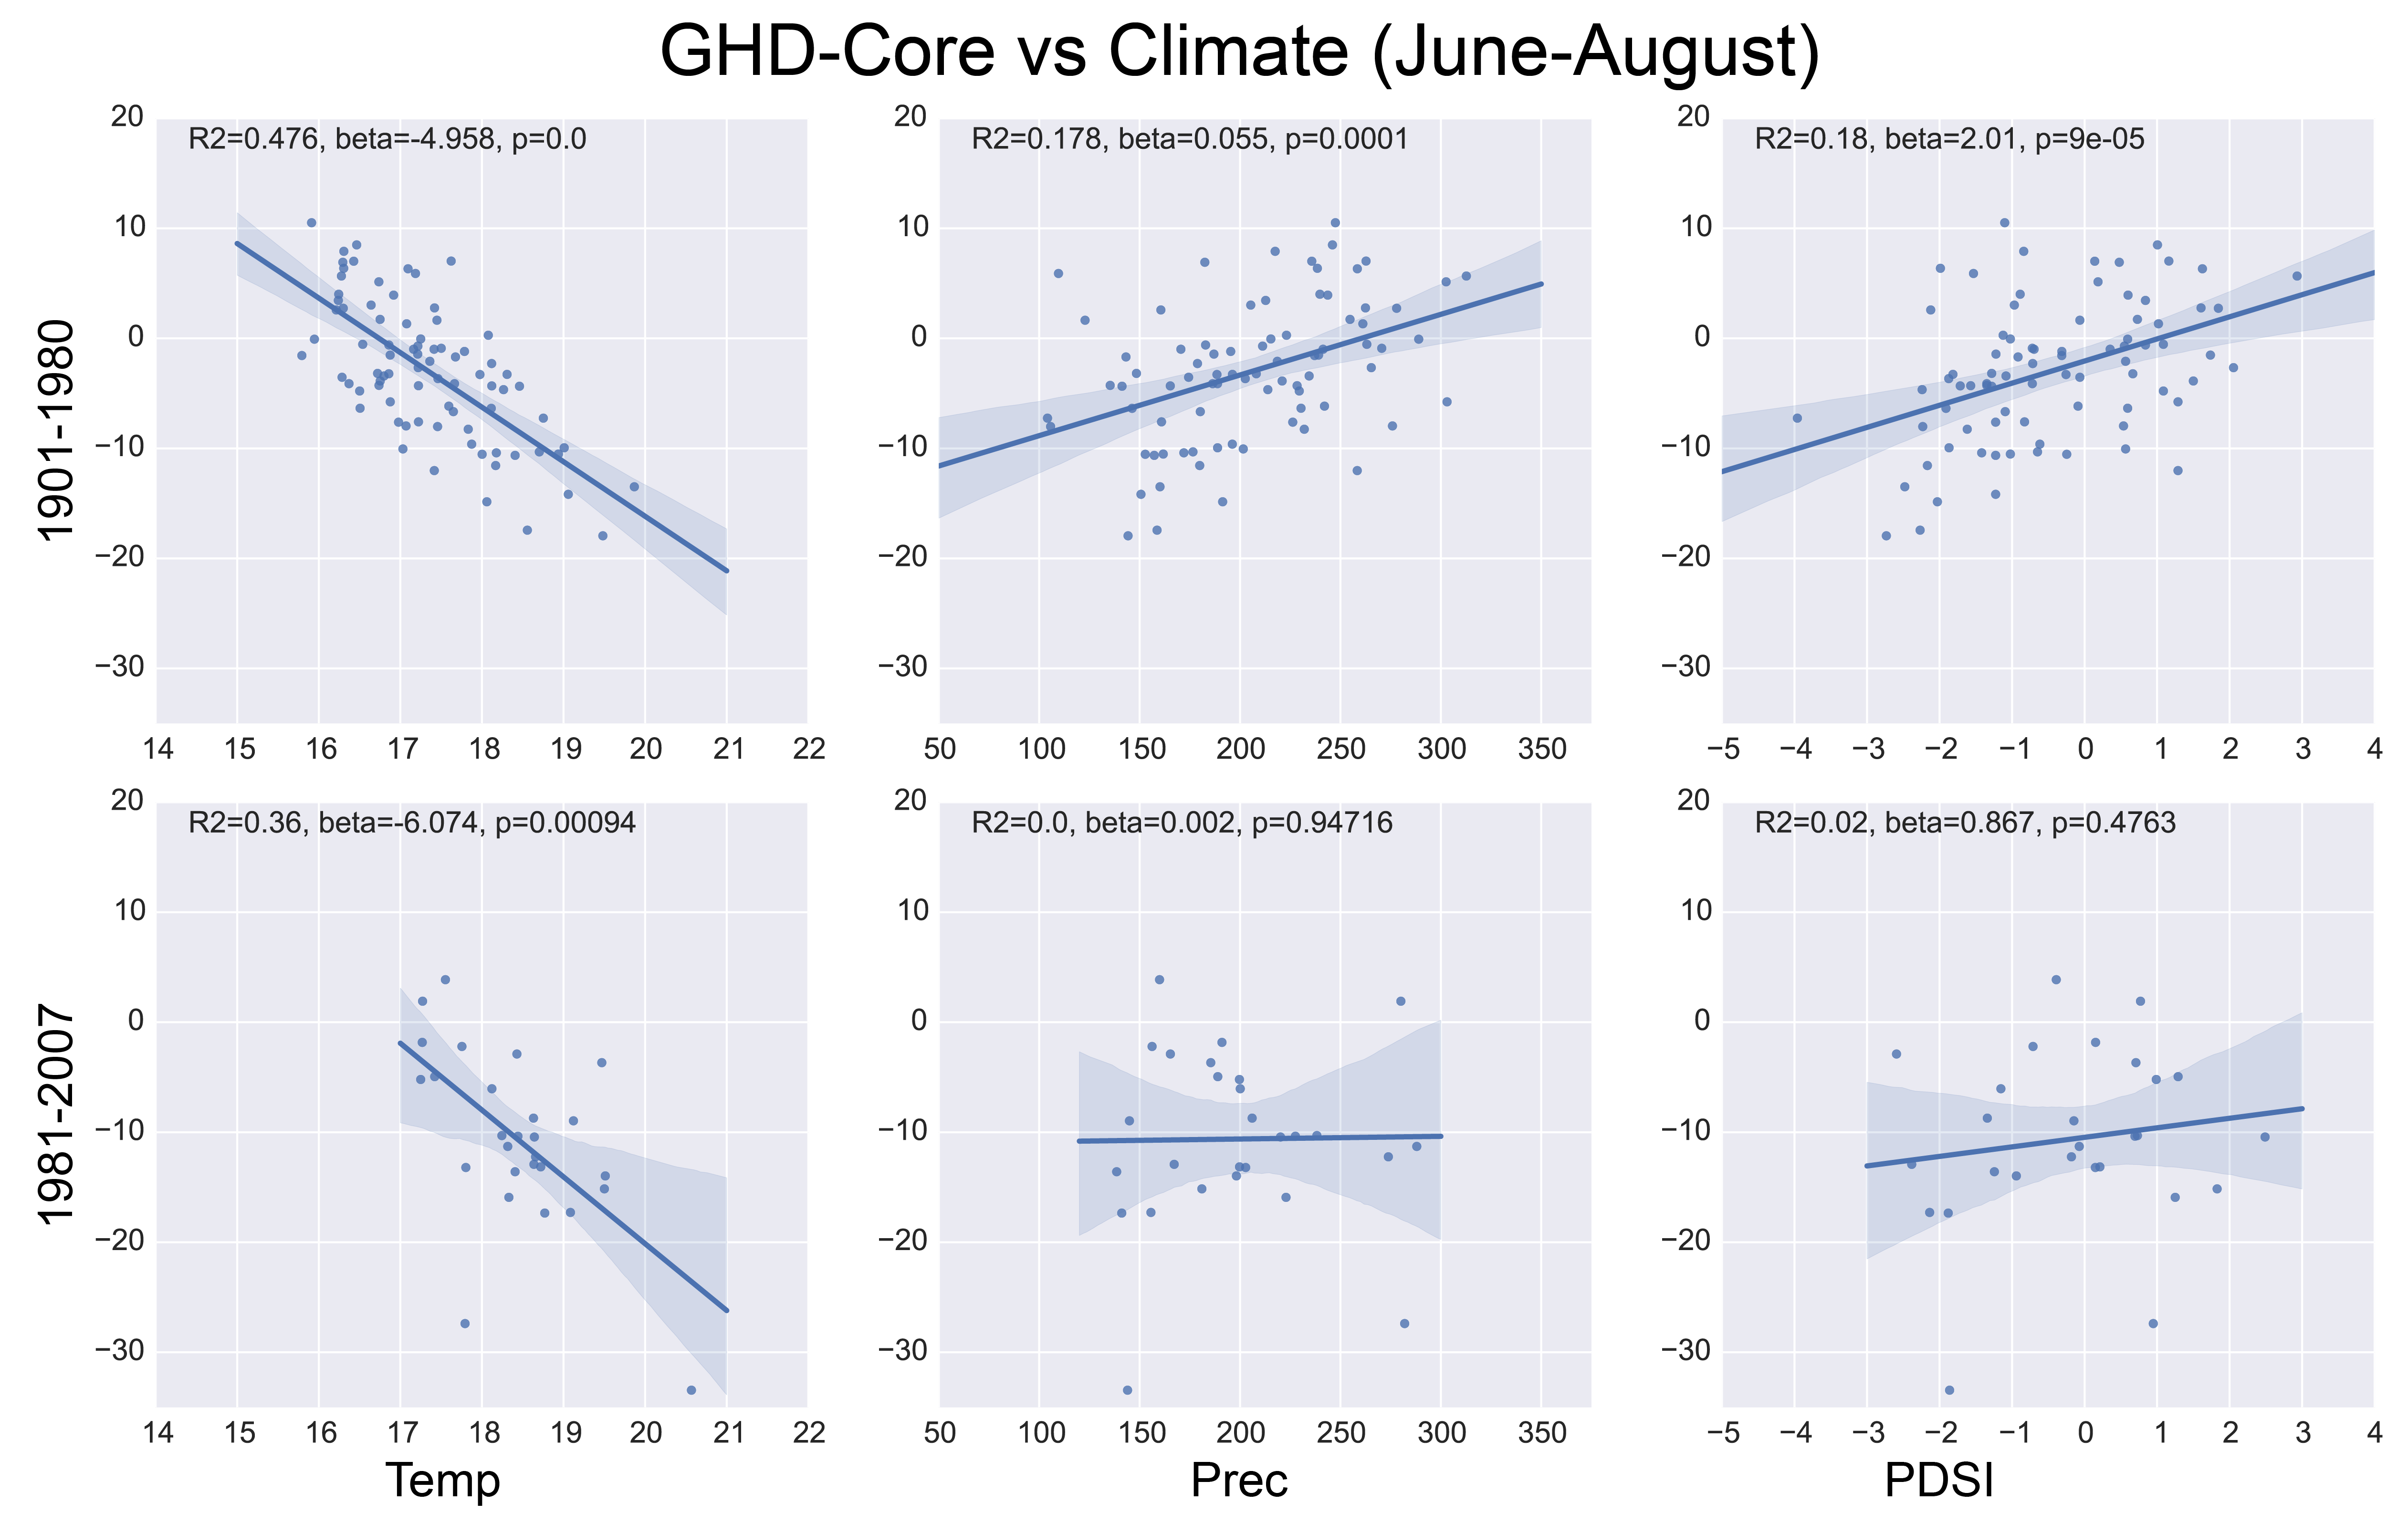
\includegraphics[width=1.0\columnwidth,scale=2]{SUPP_fig_12_JJA_clim_regplots.png}
\caption{Same as Figure 3 from the main manuscript, but for June-July-August (JJA).}
\end{figure}

\begin{figure}
\center
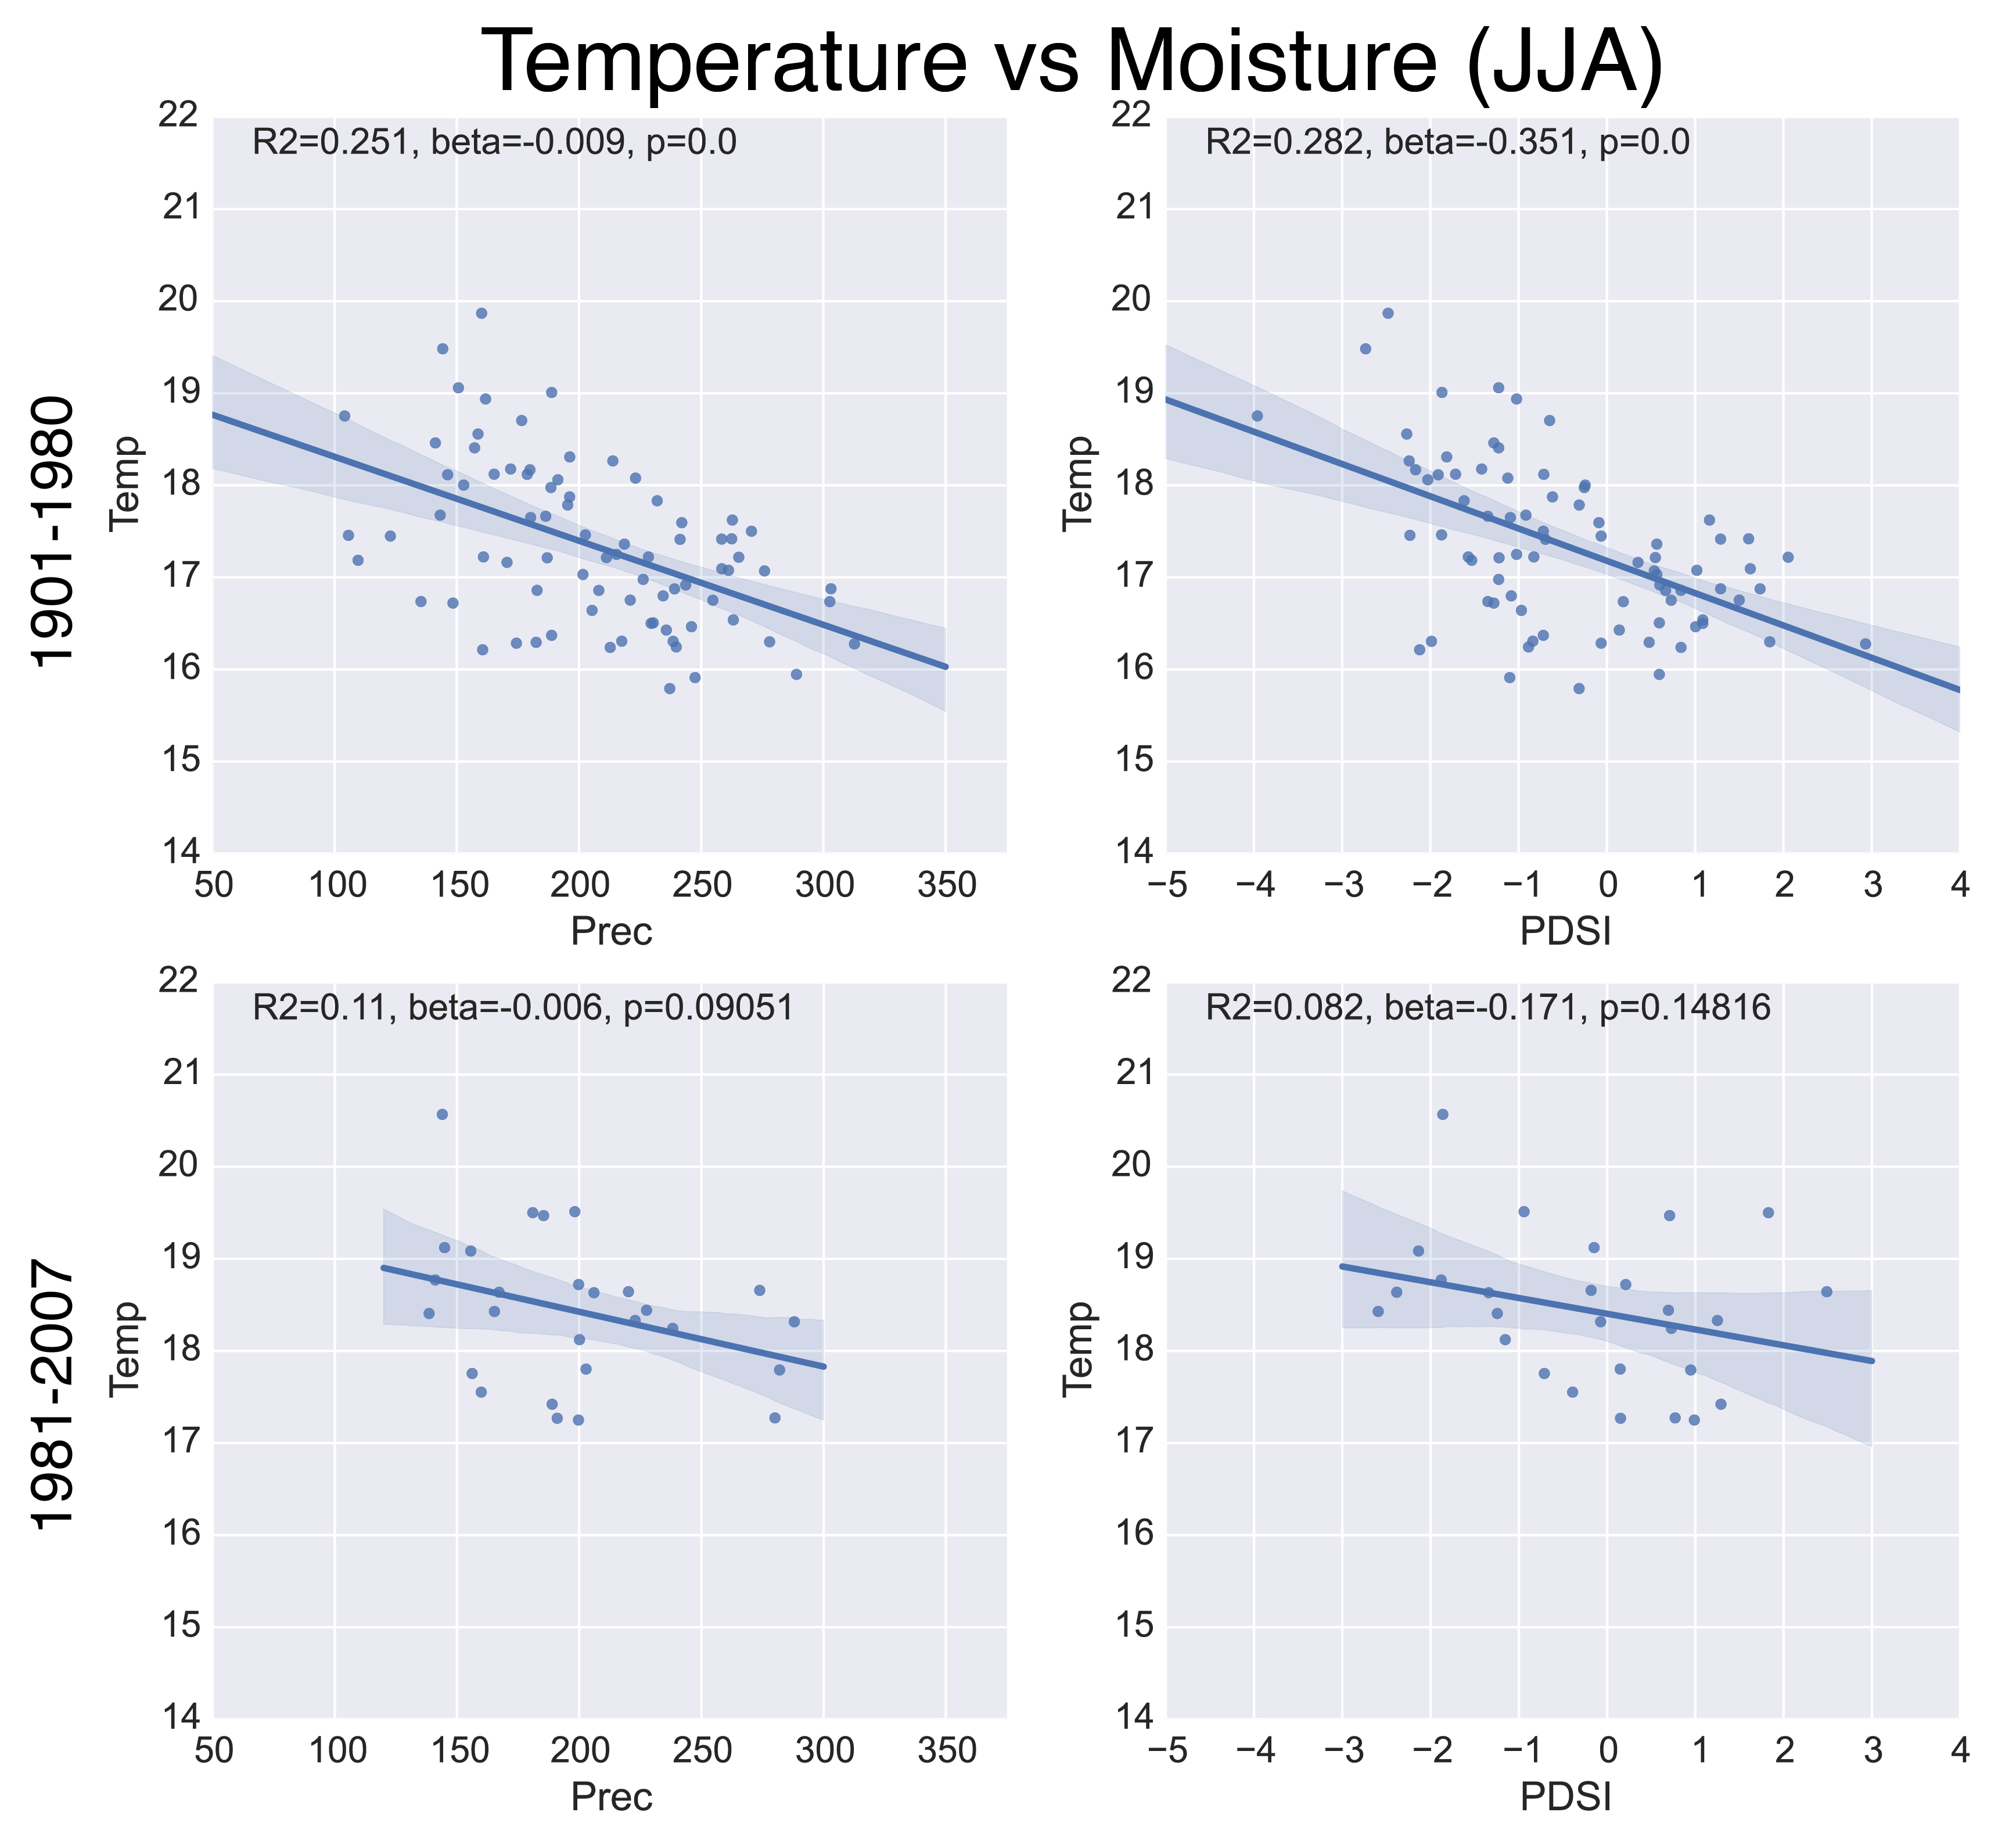
\includegraphics[width=1.0\columnwidth,scale=2]{SUPP_fig_13_temp_vs_moist_JJA.png}
\caption{Same as Supplemental Figure 11, but for June-July-August (JJA) climate. During JJA, the temperature moisture relationship is stronger over this region and, in both precipitation and PDSI, these relationships breakdown in the recent decades (1981--2007).}
\end{figure}

\begin{figure}
\center
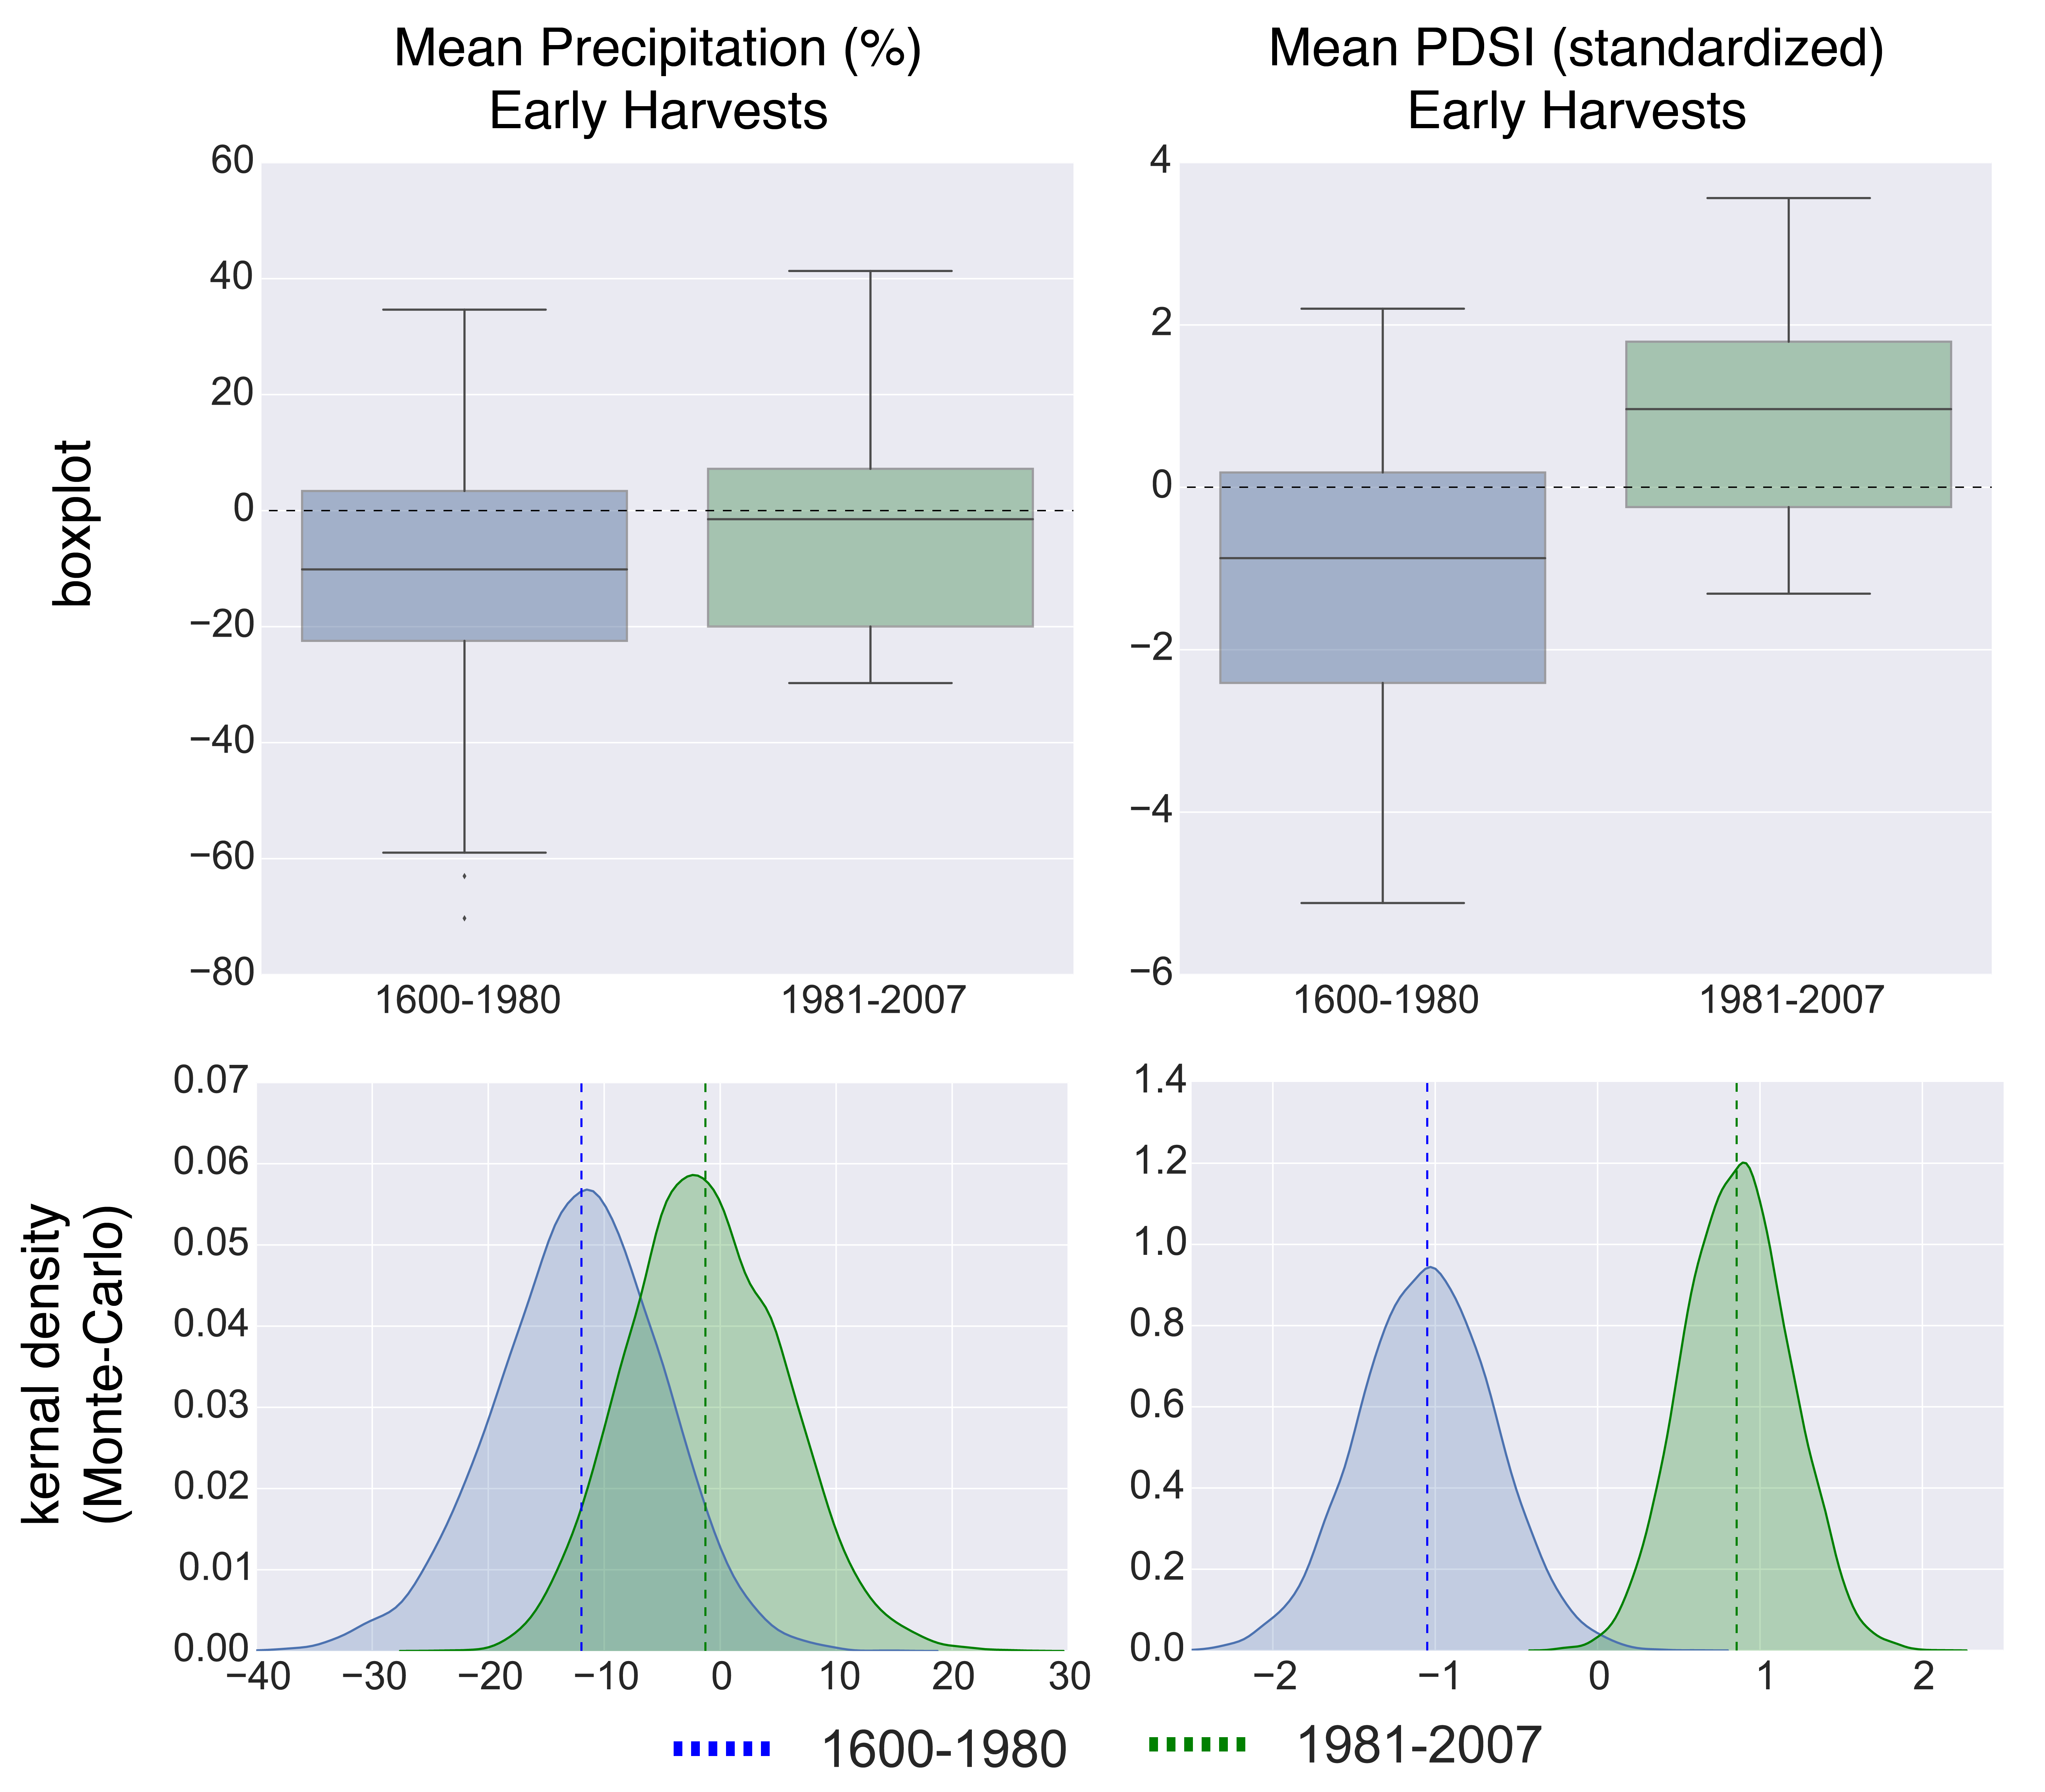
\includegraphics[width=1.0\columnwidth,scale=2]{SUPP_fig_14_JJA_boxplot_monte.png}
\caption{Top row: box plots of pooled precipitation and PDSI anomalies from the climate reconstructions for years with early harvest date anomalies in GHD-Core. Bottom row: kernel density functions of recalculated mean precipitation and PDSI anomalies associated with early harvest dates, based on 10,000 Monte-Carlo resamplings with replacement.}
\end{figure}

\end{document}









